\documentclass{sig-alternate}

%% =============================================================
\def\tool{\textsc{Clotho}\xspace}
%\def\papertitle{\tool: Program Repairing using Exception Types, Constraint
%Automata and Typestate}
\def\papertitle{CLOTHO: Saving Programs from Malformed Strings and
Incorrect String-Handling}
\def\pdfauthors{}
\def\paperkeywords{}
%% =============================================================

\usepackage{color}

\newcommand{\subparagraph}{}

% You can tweak clickable link colors here:
\definecolor{linkcol}{rgb}{0,0,1}
\definecolor{citecol}{rgb}{0,0.5,0}
\definecolor{urlcol}{rgb}{0.3,0,0}

% Make pdflatex use letter size --md
\setlength{\pdfpagewidth}{8.5in}
\setlength{\pdfpageheight}{11in}

\let\proof\relax
\let\endproof\relax

\usepackage[utf8]{inputenc}
\usepackage[T1]{fontenc}
%\usepackage{sty/microtype}

\usepackage{cite}
\usepackage{amsthm}
% \usepackage{amsmath}
% \usepackage{amsfonts}
\usepackage{ragged2e}
\usepackage{txfonts}
\usepackage{fancyhdr}
\usepackage{amssymb}
\usepackage{fancyvrb}
\usepackage{graphicx}
\usepackage{times}
\usepackage{pifont}
\usepackage[hyphens]{url}
\usepackage{xspace}
\usepackage{sty/algorithm2e}
%%\usepackage[belowskip=-10pt,aboveskip=5pt,small,labelfont=bf]{caption}
\usepackage[aboveskip=5pt,small,labelfont=bf]{caption}
\DeclareCaptionType{copyrightbox}
\usepackage[bookmarks=true,%
bookmarksnumbered=true,%
colorlinks=true,%
linkcolor=linkcol,%
citecolor=citecol,%
urlcolor=urlcol,%
hypertexnames=true,%
pdfpagelabels,
% draft
]{hyperref}


\hypersetup{%
  colorlinks=false,% hyperlinks will be black
  pdfborderstyle={/S/U/W 1}% border style will be underline of width 1pt
}

\usepackage{sty/multirow}
\usepackage{sty/flushend}
\usepackage{epstopdf}
\usepackage[small,compact]{sty/titlesec}
\usepackage[font=scriptsize]{subfig}
\usepackage{sty/wrapfig}

\usepackage{epstopdf}
\usepackage{fancybox}
\usepackage{listings}
\usepackage{xcolor}
\usepackage[normalem]{sty/ulem}
%\usepackage[]{datetime}
%\usepackage{lipsum}

\newcommand{\ignore}[1]{}
% \usepackage{rotating}

%==========================================
%Added definitions
% \usepackage{amsthm}
\theoremstyle{definition}
\newtheorem{definition}{Definition}[section]
%==========================================
%rename listing
\renewcommand\lstlistingname{Code}
%==========================================

%==========================================
%rotate column title
\usepackage{booktabs}
% \usepackage{xparse}
% \NewDocumentCommand{\rot}{O{45} O{1em} m}{\makebox[#2][l]{\rotatebox{#1}{#3}}}
%==========================================

%==========================================
%Automatic row number in table
% \usepackage{array,etoolbox}
% \preto\tabular{\setcounter{magicrownumbers}{0}}
% \newcounter{magicrownumbers}
% \newcommand\rownumber{\stepcounter{magicrownumbers}\arabic{magicrownumbers}}
%==========================================
\SetAlFnt{\small}
\SetAlCapFnt{\small}
\SetAlCapNameFnt{\small}
\SetVlineSkip{0pt}

\setlength\floatsep{5pt}
\setlength\textfloatsep{5pt}
\setlength\intextsep{5pt}

\hypersetup{
pdfauthor = {},
pdftitle = {\papertitle},
pdfkeywords = {\paperkeywords},
pdfcreator = {LaTeX with hyperref package},
pdfproducer = {pdflatex}}

\definecolor{dkgreen}{rgb}{0,0.6,0}
\definecolor{gray}{rgb}{0.5,0.5,0.5}
\definecolor{mauve}{rgb}{0.58,0,0.82}

\lstset{%frame=tb,
  captionpos=b,
  language=Java,
  aboveskip=10pt,
  belowskip=0pt,
  abovecaptionskip=5pt,
  belowcaptionskip=5pt,
  numberblanklines=false,
  showstringspaces=false,
  columns=flexible,
  basicstyle={\scriptsize\ttfamily\bfseries\color{black}},
  numbers= left,
  numbersep=5pt,
  %frame=single,
  numberstyle=\tiny\color{black},
  keywordstyle=\bfseries\color{blue},
  commentstyle=\color{dkgreen},
  stringstyle=\color{mauve},
  breaklines=true,
  breakatwhitespace=true
  tabsize=2,
  xleftmargin=2em,
  morecomment=[l]{//},
  escapeinside={<@}{@>},
}

\makeatletter
\lst@Key{countblanklines}{true}[t]%
    {\lstKV@SetIf{#1}\lst@ifcountblanklines}

\lst@AddToHook{OnEmptyLine}{%
    \lst@ifnumberblanklines\else%
       \lst@ifcountblanklines\else%
         \advance\c@lstnumber-\@ne\relax%
       \fi%
    \fi}
\makeatother

% Use a smaller font size for URLs:
\makeatletter
\def\url@myurlstyle{%
   \@ifundefined{selectfont}{\def\UrlFont{\small}}{\def\UrlFont{\small}}}
   \makeatother
\urlstyle{myurl}

% This adds ':' to the characters after which not to break URLs, and
% defines a smaller typewriter font. --cpk
% changed small to sf -- md
\def\UrlNoBreaks{\do:\do\(\do\[\do\{\do\<}%
\def\UrlFont{\small\ttfamily}
\def\UrlOrds{\do\*\do\~}%

% For referencing sections, Vern-style
\newcommand\xref[1]{\S~\ref{#1}}

% Black filled circles with white number on it
% See Comprehensive LaTeX Symbol List --cpk
\def\blackI{\ding{182}}
\def\blackII{\ding{183}}
\def\blackIII{\ding{184}}
\def\blackIV{\ding{185}}
\def\blackV{\ding{186}}
\def\blackVI{\ding{187}}

\def\first{({\it i})\xspace }
\def\second{({\it ii})\xspace }
\def\third{({\it iii})\xspace }
\def\fourth{({\it iv})\xspace }
\def\fifth{({\it v})\xspace }

% For notes to authors:
\newcommand{\note}[1]{{\textcolor{red}{[\textit{#1}]}}}

% Fine-tuning for table spacing. --cpk
\def\TblSpT{\rule[-1ex]{0pt}{0pt}}
\def\TblSpB{\rule{0pt}{2.5ex}}

% Squeezing out some space. --cpk
% http://www-h.eng.cam.ac.uk/help/tpl/textprocessing/squeeze.html
%
%\renewcommand\subfigtopskip{0pt}
%\renewcommand\subfigbottomskip{5pt}
%\renewcommand\subfigcapskip{0pt}
%\renewcommand\floatpagefraction{.9}
%\renewcommand\topfraction{.9}
%\renewcommand\bottomfraction{.9}
%\renewcommand\textfraction{.1}
%\setlength{\parskip}{0em}
%\frenchspacing


%%%%%%%%%%%%%%%%%%%%%%%%%%%%%%%%%%%%%%%%%%%%%%%%%
% \hyphenpenalty 10000
% \exhyphenpenalty 10000
\sloppy
%%%%%%%%%%%%%%%%%%%%%%%%%%%%%%%%%%%%%%%%%%%%%%%%%

\newcommand{\comment}[1]{{\color{red}#1}}
\newcommand{\code}[1]{\texttt{\bfseries\scriptsize{#1}}}
\newcommand{\mycomment}[1]{}
\newcommand{\todo}[1]{\textbf{TODO: #1}}
\newcommand{\mytab}{~~~~}
\newcommand{\sspace}{~}
\newcommand{\etal}{\textit{et al.}}
\newcommand{\eg}{{e.g.,}}
\newcommand{\ie}{{i.e.,}}
\newcommand{\lno}[1]{{\tiny{\textbf{(#1)~~}}}}

\newcommand{\java}{\textsc{Java}}
\newcommand{\soot}{\textsc{Soot}}
\newcommand{\infoflow}{\textsc{InfoFlow}}
\newcommand{\sdn}{{SDN}}
\newcommand{\verifier}{\textsc{Verifier}}
\newcommand{\validator}{\textsc{Flow\_Consistency\_ Validator}}
\newcommand{\outputs}{{\mathbb O}}
\newcommand{\stream}{{\mathbb S}}
\SetEndCharOfAlgoLine{}

%% for IEEEtran
\def\tablename{Table}

\renewcommand{\thetable}{\arabic{table}}

\newcommand*{\refname}{Bibliography}

\def\yes{\ding{51}}
\def\no{\ding{55}}

%------------------------------------------------------------------------------
%                                Space savers.
%------------------------------------------------------------------------------
% This mylist environment indents items, and saves less space than the above.
\newcounter{myctr}
\newenvironment{mylist}{\begin{list}{(\textbf{\arabic{myctr}})}
{\usecounter{myctr}
\setlength{\topsep}{1mm}\setlength{\itemsep}{0.5mm}
\setlength{\parsep}{0.5mm}
\setlength{\itemindent}{0mm}\setlength{\partopsep}{0mm}
\setlength{\labelwidth}{-2mm}
\setlength{\leftmargin}{0mm}}}{\end{list}}

% Space saving List environment for itemizing.
\newenvironment{mybullet}{\begin{list}{$\bullet$}
{\setlength{\topsep}{1mm}\setlength{\itemsep}{0.5mm}
\setlength{\parsep}{0.5mm}
\setlength{\itemindent}{0mm}\setlength{\partopsep}{0mm}
\setlength{\labelwidth}{-2mm}
\setlength{\leftmargin}{0mm}}}{\end{list}}

\newcommand{\myparagraph}[1]{\noindent{\scshape \bfseries #1.}}

%% added to remove indentation in susbsubsection for IEEEtran
% \makeatletter
% \def\subsubsection{\@startsection{subsubsection}% name
%       {3}% level
%       {\z@}% indent (formerly \parindent)
%       {0ex plus 0.1ex minus 0.1ex}% before skip
%       {0ex}% after skip
%       {\normalfont\normalsize\textbf}}% style
% \makeatother

%------------------------------------------------------------------------------
%                               Fancy header setup.
%------------------------------------------------------------------------------
%
\pagestyle{fancyplain}
\lhead{}
\lfoot{}
\chead{}
\rhead{}
\cfoot{\thepage}
%%\rfoot{{\scriptsize \today}}
\renewcommand{\headrulewidth}{0pt}

%\setlength{\intextsep}{10pt plus 2pt minus 2pt}

%% Reducing margins further -- md
%%\addtolength{\hoffset}{-0.25in}
%%\addtolength{\textwidth}{0.5in}
%%\addtolength{\voffset}{-0.25in}
%%\addtolength{\textheight}{0.4in}

% The space-saving sledgehammer. -- md
%\renewcommand{\baselinestretch}{0.95}


% \pagenumbering{arabic}

\begin{document}

%permission block
% \conferenceinfo{ESEC/FSE'15,}{August 30 -- September 4, 2015, Bergamo, Italy}
% \CopyrightYear{2015}
% \crdata{978-1-4503-3675-8/15/08}

\toappear{}

\title{\papertitle}

\numberofauthors{4}

\author{
    Aritra Dhar\xrci \\%%[4pt]
%     \email{aritra.dhar@xerox.com}
    \and
    Rahul Purandare\iiit  \\%%[4pt]
%     \email{purandare@iiitd.ac.in}
    \and
    Mohan Dhawan\ibm\iiit  \\%%[4pt]
%     \email{mohan.dhawan@in.ibm.com}
    \and
    Suresh Rangaswamy\iiit  \\%%[4pt]
%     \email{suresh1317@iiitd.ac.in}
%     \\ [4pt]
%     
    \sharedaffiliation
        \affaddr{{\xrci Xerox Research Centre India}} &
        \affaddr{{\iiit IIIT Delhi}} &
        \affaddr{{\ibm IBM Research}} \\ %%[4pt]
        \affaddr{{Bangalore, India}} &
        \affaddr{{New Delhi, India}} &
        \affaddr{\ \ \ {New Delhi, India}}
}

\maketitle

\begin{abstract}
{
%\small

Software is susceptible to malformed data originating from untrusted sources.
Occasionally the programming logic or constructs used are inappropriate to
handle the varied constraints imposed by legal and well-formed data.
Consequently, softwares may produce unexpected results or even crash.


In this paper, we present \tool, a novel hybrid approach that saves such
softwares from crashing when failures originate from malformed strings or
inappropriate handling of strings. \tool\ statically analyses a program to
identify statements that are vulnerable to failures related to associated string
data. \tool\ then generates patches that are likely to satisfy constraints on
the data, and in case of failures produces program behavior which would be close
to the expected. The precision of the patches is improved with the help of a
dynamic analysis.


We have implemented \tool\ for the \java\ \code{String} API, and our evaluation
based on several popular open-source libraries shows that \tool\ generates
patches that are semantically similar to the actual patches generated by the
programmers in the later versions. Additionally, these patches are activated
only when a failure is detected, and thus \tool\ incurs no runtime overhead
during normal execution, and negligible overhead in case of failures.

}
\end{abstract}


\category{D.2.5}{SOFTWARE ENGINEERING}
{Testing and Debugging }
[Error handling and recovery]



\keywords
{
Automatic Program Repair, 
Program Analysis,
Strings}

\section{Introduction}
\label{sec:intro}

% marker
\textcolor{red}{\textbf{Changes done}}\newline

Exception handling attributes to the response of program during runtime to some
exceptional condition encounter.
Most of the time it changes normal flow of program. In many cases exception
handling is natural part of software execution due to the nature of the
software.
An application which constantly accesses I/O which also includes share resources
may throw exception if another application blocks it.
Here in this paper we discuss and analyze java exceptions and produce repair
patch based on that. Java supports two types of exceptions :
\begin{itemize}
	
\item \textbf{Checked exception} which requires explicit \texttt{throws}
declaration at the method declaration or \texttt{try-catch} block by the
developers. Such exceptions are handled carefully as they often involves
accessing resources like network, database, file system, I/O etc.
	
\item \textbf{Unchecked exception} which does not enforce similar handing
mechanism as the former one. \texttt{java.lang.RuntimeException} and its
subclasses and \texttt{java.lang.Error} are types of unchecked exceptions.
\texttt{NullPointerException}, \texttt{ArrayIndexOutOfBound},
\texttt{ArithmeticException} are examples of common java runtime exceptions.

\end{itemize}

Oracle official documentation says that ``\emph{Here's the bottom line
guideline: If a client can reasonably be expected to recover from an exception,
 make it a checked exception. If a client cannot do anything to recover from the
 exception, make it an unchecked exception}".
 Unchecked exception, particularly runtime exceptions can be thrown from any
 point in the program making them quite unpredictable in nature.
 Due to this extensive testing phase is required to eliminate any bugs and solve
 corner cases.
 Yet many applications suffer unexpected runtime exception causing system crash
 which leads to shutdown or restart.

We find out many applications where system shutdown/restart is expensive due to
their nature.
Notable examples are air traffic control, auto pilot, life support system, smart
power grids, telephone networks, robots like UAV and rovers deployed for
surveillance, reconnaissance and knowledge acquisition in remote locations etc.
These applications are real-time sensitive and there is no room for exception
handling in such system.
Sudden crash involves risk of human life, expensive equipments and critical
services.
Other example includes web applications which uses scrips to dynamically
generate websites and interfaces as per customer preferences.
Many E-commerce websites handles queries, access and process customer and
shopping items data and commits large amount of transactions.
Sudden system crash may result in loss of precious time and data which
eventually may result in a frustrated customers move to other websites.
Many time bad or malicious code leads to some vulnerability to critical
applications and website which can be exploited by attack to orchestrate system
crash. Thought these examples cover a large variety of applications, all of them
point to some concern of \emph{availability}.

Usually, developers tests their code in series of verifications which involves
code review, static and dynamic analysis of the code, generate test cases to
cover as much potential input .Yet may corner cases can be left overlooked which
can cause runtime exceptions.
Multi-threaded applications are also susceptible to erroneous thread
interleaving. One such exception is
\texttt{java.lang.IllegalMonitorStateException}, when a thread has attempted to
wait on an object's monitor or to notify other threads waiting on an object's
monitor without owning the specified monitor. Applications under adversarial
situation should be considered where deliberate malicious input may cause it to
fail. To recover from such situation, a mechanism is needed which can predict
failure by doing invariant and symbolic analysis. Invariant analysis will detect
particular variables outside legal/safe bound. Symbolic analysis will indicate
to the potential point of failure.


In this paper we proposed two solution to suppress runtime example and ensure
system survivability. The approach consists of four primary phases

\begin{itemize}
\item \textbf{Generate input data-set} : We index user input along with the
global variables and method arguments of successful runs.
The local variables are not indexed as they can be re-generated.
These data-set is used as a reference to later executions which encounters
runtime exceptions.
Appropriate user input of previous successful run is chosen in terms of
correlation coefficient.
	
\item \textbf{Program slice for patching} : We perform static analysis prior to
running the program to determine data dependencies of the variables.
The analysis yields a dependency graph which is used to determine optimal slice
to be used as patch.
This patch is placed in catch block and executed with the values of previous
successful run while the original code is wrapped in try block.
	
\item \textbf{Determine type of exception and patching} : The characteristics of
patching is dependent on the type of runtime exception encountered by the
program. A piece of code may throws multiple types of exceptions and all of them
are handled at the time of patching by instrumenting multiple catch blocks.
	
\item \textbf{Use typestate for repairing} : Typestate analysis, sometimes
called protocol analysis defines valid sequences of operations that can be
typically modeled using Finite State Machine (FSM) where the states represent
abstract state of the program and the symbols are certain method invocations to
perform state transition. Typestates are capable of representing behavioral type
refinements like Iterators, where \emph{hasNext()} method should be called
before the \emph{next()} method call.
Typestate analysis is widely used as a safety feature to ensure a certain
sequence of operations maintains proper protocol or not.
% But this method is unconventional and investigated in the field of program
% repairing.
The documentations of the API used in the application will define the valid
typestate for repairing.
\end{itemize}

The object of the patching is to repair the problem closest to it to minimize
any collateral damage to other parts of the applications hence minimizing the
chance of unintentional data loss/corruption.

\section{Overview}
\label{sec:overview}

Ensuring correctness of a program statically is an undecidable problem. Thus
there is always a tradeoff between precision and scalability that static program
analysis must balance. Static analysis achieves high scalability by making sound
approximations, which typically leads to false positives. Complex
programming logic and data coming from diverse sources make the already hard
problem worse. As a result, successful execution of a real application can never
be guaranteed, and unexpected failures may happen. These failures often result
in applications throwing runtime exceptions, which if not handled correctly
may crash the application.

\ignore{ \begin{table}[t] \scriptsize \centering
\begin{tabular}{|l|r|r|}
\hline
\multicolumn{1}{|c|}{\textbf{Runtime Exception Type}} &
\multicolumn{1}{c|}{\textbf{Frequency}} & \multicolumn{1}{c|}{\textbf{\%}}\\
% \scalebox{0.83}
% {
\hline
\code{NullPointerException} & $34912$ & $54.94$ \\
\code{ClassCastException} & $7504$ & $11.81$ \\
\code{IndexOutOfBoundsException} & $6637$ & $10.44$ \\
\code{SecurityException}  & $5818$ & $9.15$ \\
\hline
\end{tabular}
\caption{Prominent runtime exceptions from
\texttt{stackoverflow}~\cite{stackoverflow}.}
\label{tab:stackoverlow}
% }
\end{table}
}


\lstset{language=Java, caption=Snippet from \code{fileUtils} class in Apache
Commons library. , label = snippet:exampleRepairing2}
\begin{figure}[t]
\centering
\begin{lstlisting}
public static String getPathNoEndSeparator
        (String filename) {
  return doGetPath(filename, 0);
}
private static String doGetPath
        (String filename, int separatorAdd) {
  if(filename == null) return null;
  int prefix = getPrefixLength(filename);
  if (prefix < 0) return null;
  int index = indexOfLastSeparator(filename);
  if ((prefix >= filename.length()) || (index < 0))
        return "";
  return filename.substring(prefix,
        index + separatorAdd);
}
\end{lstlisting}
\end{figure}

Code~\ref{snippet:exampleRepairing2} corresponds to methods from
\code{fileUtils} class in Apache Common IO library. The method
\code{getPathNoEndSeparator()} throws a \code{StringIndexOutOfBounds} exception,
which originates from statement \code{return filename.substring(prefix, index +
separatorAdd)} on line 13 when the method is called with parameter
\code{"/foo.xml"}.  Here, the value of \code{prefix} as returned by the method
\code{getPrefixLength} is 1. It fails to satisfy the constraint implied by the
program condition \code{prefix <= index + separatorAdd} for \code{substring}
method, which ensures that \code{beginIndex} cannot be greater than
\code{endIndex}. As a result, the exception is thrown.


\lstset{language=Java, caption=Patch for \code{fileUtils} bug in Apache Commons
library., label = snippet:exampleRepairing3, firstnumber = 13}
\begin{figure}[t]
\centering
\begin{lstlisting}
String temp = null;
try {
  temp = filename.substring(prefix, index + separatorAdd);
} catch(IndexOutOfBoundsException ex) {
  int length = filename.length;
  int t = index + separatorAdd;
  temp = filename.substring(
    getStart(prefix,t,length), getEnd(prefix,t,length));
}
return temp;
\end{lstlisting}
\end{figure}

A closer inspection of this code snippet shows that the string variable
\code{filename} invokes two methods, namely \code{length} and \code{substring}
on lines $11$ and $13$ respectively. \java\ \code{String} API documentation
specifies that \code{length} does not throw any runtime exceptions. The only
exception that this invoke statement can throw is when the receiver object
referenced by \code{filename} is \code{null}. However, the check on line $7$
indicates that this situation would not arise. The method \code{substring} may
throw \code{IndexOutOfBoundsException} exception that can potentially crash the
program. A good patch to handle this failure should take into account all of
these observations. 

Code~\ref{snippet:exampleRepairing3} presents the patch automatically generated
by \tool. This patch replaces the invoke statement on line 13 in
Code~\ref{snippet:exampleRepairing2}, which is now wrapped within a
\code{try--catch} block. The \code{catch} corresponding to
\code{IndexOutOfBoundsException}
% is added on line 15
ensures that control passes
to the catch block only when the exception is thrown. Line 20 shows two method
calls namely \code{getStart} and \code{getEnd} that are inserted by \tool. These
methods, using the knowledge about the length of \code{filename} acquired with
the help of the code on line 17, compute legally correct indexes required by
\code{substring} method to satisfy the constraint related to \code{beginIndex}
and \code{endIndex}. Method \code{substring} can now regenerate the substring
ensuring that the method call will not fail. The actual patch provided by the
developers is semantically similar to the one developed by \tool, and both
versions of the program generate the exact the same output.
% for the failed test case.

\ignore{Similarly, the patch developed by \tool\ for the bug depicted in
Code~\ref{snippet:exampleRepairing1} is semantically similar to the actual one
provided by the developers and is presented in
Code~\ref{snippet:exampleRepairing4}. Here the object referenced by the string
variable \code{temp} is regenerated after adjusting the offset and ensuring that
the constraint represented by the program condition \code{offset <= length}
would never be violated.


\lstset{language=java, caption=Patch for the Apache Log4j bug.,
label = snippet:exampleRepairing4, firstnumber =4}
\begin{figure}[t]
\centering
\begin{lstlisting}
try {
    temp = new String(chars, offset, length);
} catch(StringIndexOutOfBoundsException ex) {
    int i = chars.length;
    temp = new String(chars,
        IndexRepair.getStart(offset, length, i),
            IndexRepair.getEnd(offset, length, i));
}
priorVariables.add(temp);
\end{lstlisting}
\end{figure}
}

\ignore{\note{\tool\ performs hybrid constraint analysis to produce high-quality
patches.
This analysis ensures that the generated \code{String} objects obeying constraints imposed on them
by the program so as to exhibit a behavior that is close to the intended one. This ability of
\tool\ is illustrated by an example in
Code~\ref{snippet:constraintCollection}. Line numbers $3, 4, 5 $ and $7$ in
Code~\ref{snippet:constraintCollection} contain conditions associated with
\code{st}. The first three constraints can be collected and evaluated
statically and the last one dynamically as \code{userInput()} will return a
\code{String} object only at runtime. All of these constraints are stored in a
data structure called \textit{constraint store} for evaluation which is shown in
Figure~\ref{fig:constraint}. %\tool\ uses constraint store to evaluate
%which is described in Algorithm~\ref{algo:constraint}. More detailed process is
%discussed later in~\xref{sec:tool:stage2}.
The process of evaluation is described in Algorithm~\ref{algo:constraint} and
discussed in~\xref{sec:tool:stage2}. }
\note{Aritra: Can't we provide a real example here? It need not be an
 example from our study. Any real example will do.}
}

\section{Problem Definition}
\label{sec:definition}

Let the behavior $\mathcal{B}$ of program $\mathcal{P}$ for input $\mathcal{I}$
be a sequence of data values $\textless b_1, \ldots, b_n \textgreater$ shared
with the environment, where these values may be used to print information on
screen, access and manipulate files and databases, and exchange data with other
processes or threads. For brevity, we assume that the program is sequential.
However, our formalization and arguments can be extended to multi-threaded
programs and their behaviors.

Consider the behavior $\mathcal{B}$ to be composed of $\mathcal{B}_c = \textless
b_{1_c}, \ldots, b_{n_c} \textgreater$ and $\mathcal{B}_n = \textless b_{1_n},
\ldots, b_{n_n} \textgreater$, where elements in $\mathcal{B}_c$ consist of
critical values that form core functionality of the program, while elements in
$\mathcal{B}_n$ are noncritical values with respect to the core functionality of
the program.
% We consider behaviors of the two programs, $\mathcal{P}$ and
% $\mathcal{P}'$, equivalent if their critical components are identical for same
% program inputs. Formally, $\mathcal{P} \equiv \mathcal{P}' \iff$
% ($\mathcal{B}_c
% = \mathcal{B}'_c \land \mathcal{I} = \mathcal{I}'$). In other words, for
% equivalent program behaviors their noncritical behaviors do not matter.
%  
% Let $\mathcal{B}_{I_f}$ be the behavior for $\mathcal{P}$ under failure input
% $\mathcal{I}_f$. and let the data element that correspond to the failure does
% not belong to $\mathcal{B}_{{I_f}_c}$. Let the element be $b_{m_n}$.
% 
% Let p be an element of P which results in a failure under cer-
% tain input I f . Let the intended behavior of P under this input be
% BI f , and let the data element that correspond to the failure does not
% belong to BI f c . Let the element be bmn .
%  
% In this work, we restrict our approach to data values that are strings.
% 
If $\mathcal{B}_{\theta}$ is the behavior for $\mathcal{P}$ under failure input
$\theta$, then our approach attempts to
% i) find a minimal $p$ that was associated with the failure,
% ii) ensures that $b_{m_n} \not\in \mathcal{B}_{{I_f}_c}$,
develop a program patch to convert $\mathcal{P}$ to $\mathcal{P}'$,
% while ensuring that:
such that 
% \begin{mybullet}
%  \item
 $\mathcal{P}'$ does not violate the core behavior of $\mathcal{P}$ under
failure, \ie\ $\mathcal{B}'_{\theta_c}$ is same as the intended behavior
$\mathcal{B}_{\theta_c}$.
% , and
%  \item
Note that resulting behavior $\mathcal{B}'_{\theta_n}$ may not be
equivalent to $\mathcal{B}_{\theta_n}$.
% is close to the intended
% behavior $\mathcal{B}_{\theta_n}$. In other words, the difference between
%  $\mathcal{B}'_{\theta_n}$ and 
% $\mathcal{B}_{\theta_n}$ is within limits acceptable to the programmer.
% \end{mybullet}

\ignore{the reviewers are not happy with the informal notion of "close to" or "acceptable".
The changes I have made still do not address this issue convincingly. If we cannot
come up with a good solution to this problem, we might say
that formal definition of acceptance criteria and its enforcement is future work. Please
comment on this. 
}

\ignore{\note{I removed the offending text. Does it read better? -- md. Made
another minor change. - Rahul}}

% \subsection{Goals}
% \label{sec:tool:goals}

In this work, we restrict our approach to string data values. We identify the
broad design goals for a technique to automatically repair malformed strings or
incorrect handling of strings as follows:

% i) identifies the statements which might be vulnerable to string-related
% errors,
% and are less critical to the functionality of the application such that
% suboptimal behavior might be acceptable,
% iii) generates patches by identifying constraints on the string data and if
% required, tweaks \code{String} API  parameters to regenerate legally correct
% string data,
% iv) optimizes the number of statements to be patched by retaining only the
% ones
% that need to be protected,

\myparagraph{(i) High patch fidelity} We require that the patched program must
preserve the intended program behavior, \ie\ the patch must be precise, and
should not induce any undesirable control flows in the repaired program. 
This goal naturally follows from the problem definition. However, we set two
more goals associated with the security and performance of the technique.

\myparagraph{(ii) Non-invasive instrumentation} We require that the technique
must ensure no side-effects (aside from optimally repairing objects) during
normal program execution, and activate patches only when the program is
guaranteed to crash.

\myparagraph{(iii) Low system overhead} We desire that the patched program must
incur no runtime overhead during normal program execution, and only negligible
overhead in case of failures.

% We next present in detail techniques and algorithms to produce patches under
% more complex scenarios.
% Our study presented in \xref{sec:results} suggests that majority of
% the string generation scenarios in practice are less complex.

\section{\tool}
\label{sec:design}

\begin{figure}[t]
\centering
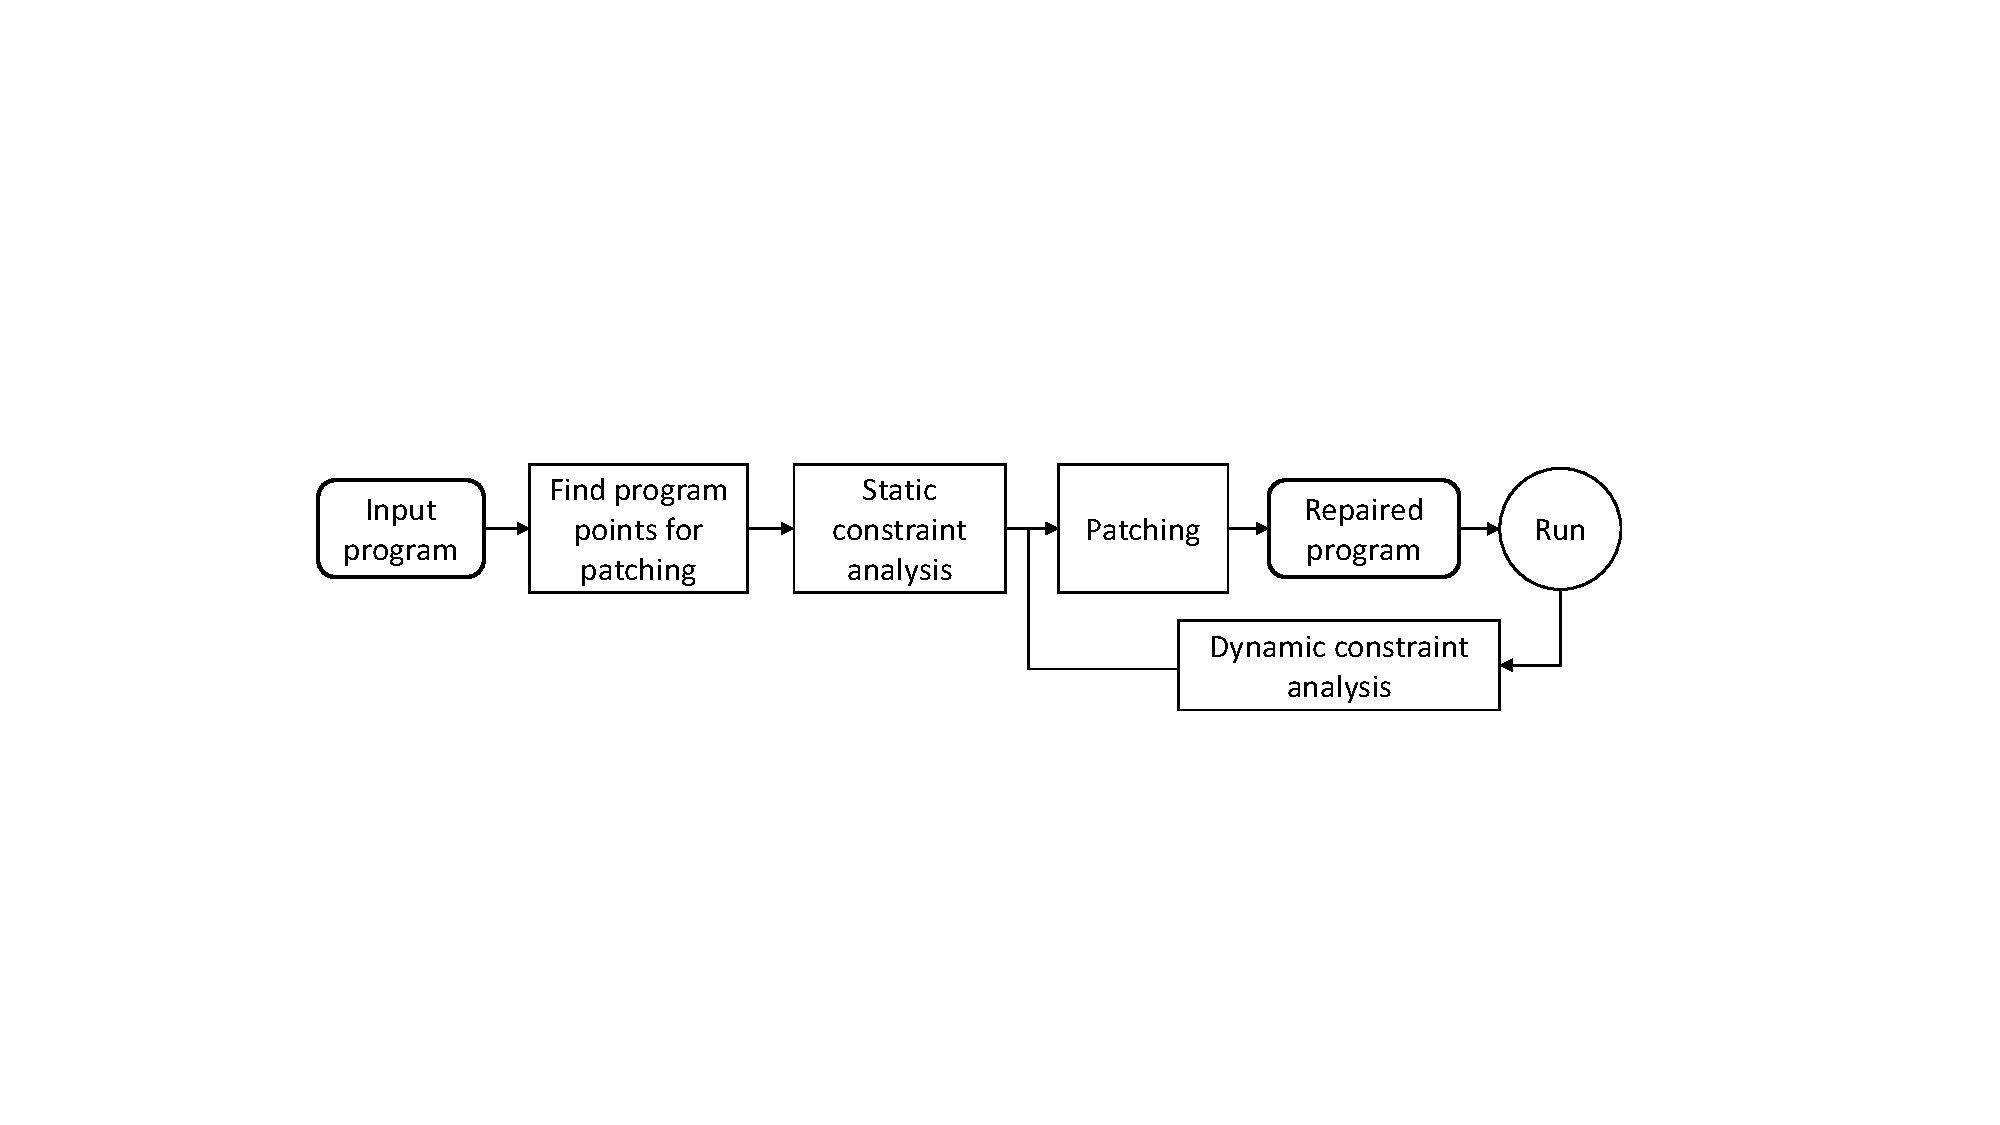
\includegraphics[scale=.38]{images/NewDesignDiagram.pdf}
\caption{\tool\ workflow.}
\label{fig:overallDesign}
\end{figure}

\myparagraph{\underline{Key Idea}} \tool\ leverages a combination of program 
analysis techniques to precisely identify program instrumentation points, and
builds upon custom algorithms to generate targeted, high quality patches for
repairing programs with potential runtime exceptions, while still satisfying
goals mentioned in \xref{sec:definition}.

Figure~\ref{fig:overallDesign} shows \tool's workflow, which involves three
main stages. First, \tool\ uses program analysis techniques to precisely
identify points of interest, \ie\ \code{string} objects or API arguments that
must be repaired to prevent runtime exceptions. In the second stage, \tool\ leverages
custom algorithms to generate relevant patches. Specifically, \tool\ performs
intra-procedural static and dynamic analyses to identify and evaluate
constraints on the string objects under consideration. Third, \tool\ uses the
constraints evaluated in the earlier stage to programatically generate and embed
patches inside \texttt{catch} blocks to ensure that they do not get activated
during normal program execution.

\subsection{Precise Identification of Instrumentation Points}
\label{sec:tool:stage1}

In this stage, \tool\ leverages a combination of program analyses to accurately
determine the minimum set of points of interest where instrumentation is
required to repair. We list several techniques below that help \tool\ achieve
precision.

\myparagraph{(i) Taint analysis} The main purpose of taint analysis is to
broadly identify which program statements can be patched (possibly even
suboptimally) without affecting the program control flow, \ie\ affect only
objects that are generated and stay within the application throughout their
lifetime. While this principle is not a binding constraint, it ensures that
\tool's repairing mechanism does not adversely affect critical program behavior.
We specify a generic set of sensitive sources and sinks for each input program,
to identify critical program paths where repaired \code{String} objects
(possibly suboptimal) must not flow. For example, \tool\ does not repair
statements that lie along a control flow path leading to an I/O sink, like file
system, console, network, GUI, etc.

\begin{table}[t]
\centering
\caption{Common sensitive sources in \java.}
\scriptsize
\begin{tabular}{|l|l|}
\hline
\multicolumn{1}{|c|}{\textbf{Class}} & \multicolumn{1}{c|}{\textbf{Source}}\\
\hline
\code{java.io.InputStream} & \code{read}\\
\code{java.io.BufferedReader} & \code{readLine}\\
\code{java.net.URL} & \code{openConnection}\\
\code{java.util.Scanner} & \code{next}\\
\code{javax.servlet.ServletRequest} & \code{getParameter}\\
\code{org.apache.http.HttpResponse} & \code{getEntity}\\
\code{org.apache.http.util.EntityUtils} & \code{toString}\\
\code{org.apache.http.util.EntityUtils} & \code{toByteArray}\\
\code{org.apache.http.util.EntityUtils} & \code{getContentCharSet}\\
\hline
\end{tabular}
\label{table:TaintSources}
\end{table}

\begin{table}[t]
\centering
\caption{Common sensitive sinks in \java.}
\scriptsize
\begin{tabular}{|l|l|}
\hline
\multicolumn{1}{|c|}{\textbf{Class}} & \multicolumn{1}{c|}{\textbf{Sink}}\\
\hline
\code{java.io.FileOutputStream} & \code{write}\\
\code{java.io.OutputStream} & \code{write}\\
\code{java.io.PrintStream} & \code{printf}\\
\code{java.net.Socket} & \code{connect}\\
\code{java.io.Writer} & \code{write}\\
\hline
\end{tabular}
\label{table:TaintSinks}
\end{table}

The taint analysis module takes as input the compiled byte code intended to be
repaired, and generates a control flow graph identifying program statements that
lie along paths from sensitive sources to sensitive sinks. Since, \tool\ targets
\code{String} objects in particular, it must support taint propagation for all
\java\ APIs that support string manipulation, including \code{StringBuffer} and
\code{StringBuilder}.
\tool\ makes a default, conservative assumption that all objects
leaving the system have potential to trigger unintended behavior. Thus, all
\code{String} objects (whether generated or assigned)
that lie along the tainted path from a sensitive source to a sensitive sink are
marked as \textit{unsafe} to patch. Subsequently, \tool\ does not repair such
\code{String} objects.

\tool's configuration further enables developers to specify their own sets of
sensitive sources and sinks, and exclude specific tainted paths.
Tables~\ref{table:TaintSources} and \ref{table:TaintSinks} list common
sensitive sources and sinks for several classes in \java.

\myparagraph{(ii) Call graph analysis} \tool\ leverages call graph analysis to
further improve the precision for finding instrumentation points. Although
unlikely, it is possible that the developers may themselves handle code that
raises runtime exceptions. \tool\ must not instrument program points that
are explicitly handled by the developers, since repairing such statements
would definitely alter the intended control flow.

Checked runtime exceptions may be placed in the (i) same method, or (ii)
upstream in the call chain. While handling the former scenario is trivial,
\tool\ handles the latter case by identifying all possible call chains (in
the \textit{call graph}) involving the concerned method using reverse breadth
first search, and determining ancestor methods where the call site was wrapped in
\code{try-catch} block of compatible exception type.

\myparagraph{(iii) Reaching definitions analysis} Taint and call graph analyses
together provide a set of program points to be instrumented with the
patch. However, this set can be further pruned. \tool\ performs \textit{reaching
definitions} analysis to skip marked statements if
(i) the \code{String} variables contained in such statements have already been
patched upstream in the method, and (ii) the variables have not been redefined along any
path that originates from the patched statement. This analysis further reduces
instrumentation points in a program.

\subsection{Patch Generation}
\label{sec:tool:stage2}

The output from the first stage is essentially a set of program points,
typically bytecodes or some other intermediate representation, denoting
\code{String} objects or APIs that are safe to repair. Once these
instrumentation points have been identified, \tool\ determines the
possible patches that can be applied to each of them. Specifically, a program
patch constitutes a set of constraints on either the \code{String} object or the
parameters to the \code{String} API under consideration, such that the new
repaired \code{String} object that is generated satisfies all constraints. Thus
the patched program does not throw any runtime exceptions.

\tool's patch generation mechanism involves two main parts (i) constraint
collection and evaluation, and (ii) code generation. We now describe \tool's
patch generation mechanism in detail. 


\begin{table}[t]
\centering
\caption{Constraints involving \code{Strings}.}
\scriptsize
\setlength{\tabcolsep}{2.5pt}
\begin{tabular}{|c|c|c|c|c|c|c|c|}
\hline
Min length($L$) & Max length($L$) & Prefix $1$ & $\ldots$ & Prefix$L$ & Contain
$1$ & $\ldots$ & Contain $L$\\
\hline
\end{tabular}
\label{table:constraint}
\end{table}

%now the image is in table form
\ignore{
\begin{figure}[t]
\centering
%% change the font size in the img; make it min len, max len
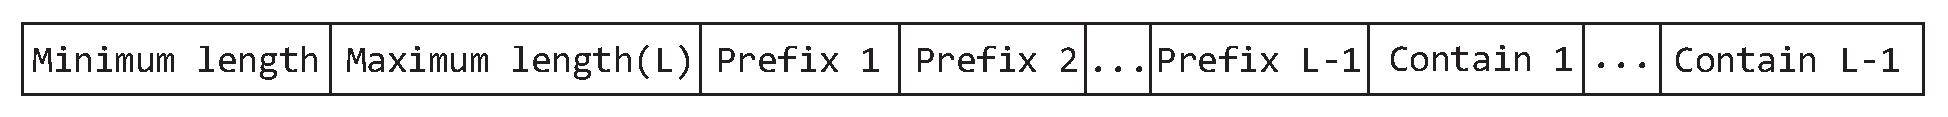
\includegraphics[width=\linewidth]{images/constraint.eps}
\caption{Constraints involving Strings.}
\label{fig:constraint}
\end{figure}
}
\myparagraph{Constraint collection and evaluation} \tool\ leverages a hybrid
approach to collect all possible constraints that must be satisfied, and thus
generates a high quality patch to repair the program. A constraint on a
\code{String} object is defined as a set of permissible values that uniquely
define the string. \tool\ uses a \textit{constraint store} to maintain a set that 
includes constraints on minimum and maximum
lengths, along with a set of permissible prefixes and substrings, as shown in
Table~\ref{table:constraint}.

\begin{algorithm}[t]
\scriptsize
\DontPrintSemicolon
\KwData{Control flow graph $CFG$ for program $P$}
\KwResult{Patched program $P'$}
\Begin
{
 \For{$\forall$ node $N \in CFG$} {
  Statement $S$ in node $N$\\
  \lIf{$S$ contains \code{String} API call} {\\
  	\mytab $str \longleftarrow$ \code{String} reference on $S$
  	
  	\lIf{$S$ can throw \code{RuntimeException}} {\\
  	  \mytab Exception class $EC \longleftarrow$ \code{RuntimeException} of
$S$\\
          \mytab $CES_{str} \longleftarrow$ all conditional statement in $P$ on
$str$\\
 \mytab  \code{/* Constraint collection for str */}\\
  	  \mytab $CS_{str} \longleftarrow$ output of
Algorithm~\ref{algo:constraintCollection}$(CES_{str})$\\

  		\mytab \lIf{$str$ have sufficient constraints in $CS_{str}$} {\\
  		
  		 \mytab  \code{/* Constraint evaluation for str */}\\
  			\mytab \mytab $str \longleftarrow$ output of
Algorithm~\ref{algo:constraint}$(CS_{str})$
  		}
  		
  		\mytab \lElse {\\
  			\mytab \mytab \code{/*Repair by parameter tweaking*/}\\
  			\mytab \mytab $str \longleftarrow$ output of
  			Algorithm~\ref{algo:stringPatchParametr}$(S)$ 
  		}
  		
  		
  		\mytab $S'\longleftarrow$ Modify $S$ with $str$ \\
  		\mytab Put $S$ in try block\\
  		\mytab Put $S'$ with patched $str$ in catch block \\
  		\mytab with the exception class $EC$	
    }
    \vspace{-2em}
  }
 }
}
\caption{Static patching strategy for \code{String} objects.}
\label{algo:patchingStrategy}
\end{algorithm}

\begin{algorithm}[t]
\scriptsize
\DontPrintSemicolon
\KwData{Control flow graph $CFG$ for program $P$}
\KwResult{Patched program $P'$}
\Begin
{
 \For{$\forall$ node $N \in CFG$} {
  Statement $S$ in node $N$\\
  \lIf{$S$ contains \code{String} API call} {\\
  	\mytab $str \longleftarrow$ \code{String} reference on $S$
  	
  	\lIf{$S$ can throw \code{RuntimeException}} {\\
          \mytab $CES_{str} \longleftarrow$ all conditional statement in $P$ on
$str$\\
 
 \mytab  \code{/* Constraint collection for str */}\\
  	  \mytab $CS_{str} \longleftarrow$ output of
Algorithm~\ref{algo:constraintCollection}$(CES_{str})$\\

  		\mytab \lIf {$S$ encountered exception} {\\
  		
  		\mytab \mytab \lIf{$str$ have sufficient constraints in
$CS_{str}$} {\\

\mytab\mytab \code{/* Constraint solving for str */}\\
                        \mytab \mytab \mytab $str \longleftarrow$ output of
Algorithm~\ref{algo:constraint}$(CS_{str})$
  		} \mytab \mytab \lElse {\\
  		
  		\mytab\mytab\mytab  \code{/* Parameter tweaking */}\\
  		        \mytab \mytab \mytab $str \longleftarrow$ output of
Algorithm~\ref{algo:stringPatchParametr}$(S)$
  		}
  		}
		\vspace{-4em} 
    }
  }
 }
}

\caption{Dynamic patching strategy for \code{String} objects.}
\label{algo:patchingStrategyDynamic}
\end{algorithm}

The hybrid approach has a static component that makes a forward pass over the
program to collect constraints on \code{String} objects, such as their length or
prefix. \tool\ invokes the dynamic component if there are constraints such that
the constraint set cannot be evaluated. In such scenarios, \tool\ (i) generates
a patch that itself dynamically collects constraint information, (ii) augments
it with the previously collected static constraint details, and (iii) evaluates
these constraints on the fly to generate repaired \code{String} objects, which
do not cause the program to throw runtime exceptions. \tool\ propagates
constraints to ensure that the static constraint collection works correctly if
the conditional statements involve any variables that are redefined during the
collection and can be calculated statically. \tool\ only collects constraints
that are directly associated to \code{String} objects.
Algorithms~\ref{algo:patchingStrategy} and~\ref{algo:patchingStrategyDynamic}
give an overview of this hybrid approach.

\begin{algorithm}[t]
\scriptsize
\DontPrintSemicolon
\KwData{Set of conditional statement on string $str$}
\KwResult{Constraint set $CS_{str}$}
\Begin
{
  \For{Conditional statement$ \leftarrow i$, $\forall i \in CS_{str}$}
  {
   $i \Rightarrow str\ *\ OP$ \code{/*where $*$ is the binary operator*/}\\
   \lIf{$*$ is $==$} {\\
   \mytab $maxlength_{str} \longleftarrow OP$\\
   \mytab $minlength_{str} \longleftarrow OP$
   } \lElseIf {$*$ is \textgreater\ {\bf OR} $*$ is $\ge$} {
    $minlength_{str} \longleftarrow OP$
   } \lElseIf {$*$ is \textless\ {\bf OR} $*$ is $\le$} {
    $maxlength_{str} \longleftarrow OP$
   } \lElseIf {$*$ is Prefix Check} {
    $\textit{PrefixSet}_{str} \cup OP$
   } \lElseIf {$*$ is Contains Check} {
    $\textit{ContainSet}_{str} \cup OP$
   }
  }
}
\caption{Constraint collection for \code{String} objects.}
\label{algo:constraintCollection}
\end{algorithm}


\lstset{language=Java, caption=Static and dynamic constraint
collection example, label = snippet:constraintCollection, firstnumber =1}
\begin{figure}[t]
\begin{lstlisting}
void foo(){
  String st = "test String";
  if(st.length == 5) {/*do something*/}
  if(st.startsWith("ab")) {/*do something*/}
  if(st.startsWith("abcd")) {/*do something*/}
  /*userInput() accepts String input from console*/
  if(st.contains(userInput())){/*do something*/}
  st = st.substring(7, 10); /*Potential failure*/
}
\end{lstlisting}
\end{figure}


\begin{figure}[t]
\centering
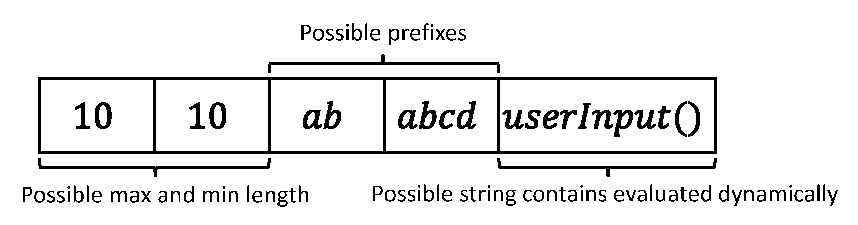
\includegraphics[width=2.5in]{images/ConstraintExample.eps}
\caption{Constraint store for Code~\ref{snippet:constraintCollection}}
\label{fig:constraintExample}
\end{figure}

\begin{mylist}

 \item \textbf{Static constraint collection}: \tool's static constraint
collection phase identifies all constraints.
Algorithm~\ref{algo:constraintCollection} briefly describes the steps to
populate the constraint store. Specifically, \tool\ \ignore{iterates over all
program code} identifies and analyzes conditional statements involving string
objects \ignore{of the form} such as \code{if (st.length() == $5$)}. It
considers only those constraints that the object must satisfy to ensure control
flows through one of the \textit{normal} branches of the conditional. A normal
branch is one that does not represent erroneous control flow. For example, a
branch that encounters a statement \code{System.err.print()} would represent an
erroneous control flow. \ignore{In other words, \tool\ only considers the
conditional expressions in the branches that do not involve any exceptions or
error paths.}

Code~\ref{snippet:constraintCollection} shows a string variable with several
constraints as defined by the \code{if} statements on lines $2$-$5$. The first
three constraints are static as all of them can be evaluated at the compilation
time. By analyzing these statements, \tool\ populates the constraint store
depicted in Figure~\ref{fig:constraintExample}. \ignore{Note that \tool\ also evaluates $OP$ (in
Algorithm~\ref{algo:constraintCollection}) when collecting constraints, in case
$OP$ is a composite mathematical expression $f(x,y,z,...)$, such as $x + y * z$,
where all $x$, $y$ and $z$ are known to be numeric.}\ignore{ When collecting
constraints, \tool\ also evaluates composite mathematical expressions, such as
$x + y * z$, where all $x$, $y$ and $z$ are numeric (see
Algorithm~\ref{algo:constraintCollection}).}

\begin{algorithm}[t]
\scriptsize
\DontPrintSemicolon
\KwData{String object \textit{Str} and constraint set $CS$.}
\KwResult{String object \textit{Str} such that $\forall i \in CS$, $Str$ satisfies $i$}
\Begin {
    $CS_{\textit{Str}} \longleftarrow$ Get the constraint set for \textit{Str}\\
    $MinLength \longleftarrow CS_{\textit{Str}}[0]$\\
    $MaxLength \longleftarrow CS_{\textit{Str}}[1]$\\
    $\textit{PrefixSet}_{\textit{Str}} \longleftarrow CS_{\textit{Str}}[2 \rightarrow MaxLength + 1]$\\
    $\textit{ContainSet}_{\textit{Str}} \longleftarrow CS_{\textit{Str}}[MaxLength +2  \rightarrow
2*MaxLength + 1]$\\

    \For{$C \in \textit{PrefixSet}_{\textit{Str}}$} {
        \lIf{$C$ is Empty} {\\
          \mytab continue
        }
        
        $\textit{PrefixLength} \longleftarrow$ {\bf LENGTH OF} $C$\\
        
        \lIf{\textit{PrefixLength} is Maximum $\in \textit{PrefixSet}_{\textit{Str}}$} {\\
          \mytab  Use $C$ to construct $\textit{Str}$
        }
    }

    \For{$C \in \textit{ContainSet}_{\textit{Str}}$} {
        \lIf{$C$ is Empty {\bf OR} $C \in \textit{Str}$} {\\
          \mytab  continue
        }
        $\textit{Str} \leftarrow \textit{Str}$ {\bf APPEND} $C$
    }
    return $\textit{Str}$
}
\caption{\code{String} object constraint evaluation.}
\label{algo:constraint}
\end{algorithm}

 \item \textbf{Dynamic constraint collection}: The constraint set is populated
at the end of the static phase. \tool\ leverages Algorithm~\ref{algo:constraint}
to evaluate these constraints and determine the potential safe values of the
\code{String} object under consideration. However, there are scenarios where
there exist potentially conflicting constraints or no permissible values of the
constraints can be calculated statically.

\ignore{
\lstset{language=Java, caption=Code requiring dynamic string constraint
evaluation., label =
snippet:exCode1, firstnumber =1}
\begin{figure}[t]
\begin{lstlisting}
void foo() {
  String st = Input(); /* user input */
  if (st.length() == 5) {/* do something */}
  if (st.contains(Input())) {/* do something */}
  st = st.substring(7, 10);
}
\end{lstlisting}
\end{figure}
}

\lstset{language=Java, caption=Dynamic constraint collection and evaluation
for code \ref{snippet:constraintCollection}., label =snippet:exCode2,
firstnumber =1}
\begin{figure}[!htb]
\begin{lstlisting}
String st = "test String";
ConstraintStore.updateLength("<foo()>", st, 5);
/*Executes if there is an exception over st*/
st = GenerateStringStatic.init("<foo()>", st);
if(st.length == 5) {}
if(st.startsWith("ab")) {/*do something*/}
ConstraintStore.updatePrefix("<foo()>", st, "ab");
st = GenerateStringStatic.init("<foo()>", st);
ConstraintStore.updatePrefix("<foo()>", st, "abcd");
st = GenerateStringStatic.init("<foo()>", st);
if(st.startsWith("abcd")) {/*do something*/}
String temp = Input();
ConstraintStore.updateSet("<foo()>", st, temp);
st = GenerateStringDynamic.init("<foo()>", st);
if(st.contains(temp){/*do something*/}
\end{lstlisting}
\end{figure}

For example, function \code{foo} in Code~\ref{snippet:constraintCollection}
performs a series of checks on a user-entered string \code{st} before computing
a substring on it. Since the constraints on \code{st} cannot be completely
collected and evaluated statically, \tool\ instruments the code with statements
to dynamically collect constraint information, augments them with previously
known static constraints, and evaluates these constraints at runtime.
Specifically, \tool\ instruments the bytecode with constraint collection code
just before the conditional statements under consideration.
Code~\ref{snippet:exCode2} depicts the example in
Code~\ref{snippet:constraintCollection} after \tool's instrumentation. When the
constraints in the source are complex, \tool\ relies on its base framework to
simplify them and then evaluates only the ones that are related to strings.

\end{mylist}

\subsection{Code generation}
\label{sec:tool:stage2:generation}

Code generation is done either statically or dynamically depending on how
the constraints are evaluated. In either scenario, a key component of code
generation is \textit{object repairing}. Additionally, in certain cases
where constraints cannot be satisfied, either statically or dynamically or
both, \tool\ resorts to \textit{parameter tweaking}.

\begin{mylist}

 \item \textbf{Object repairing}: \tool\ generates the code for the repaired
object under consideration after all the constraints have been collected and
evaluated. If the constraints are resolved statically, then \tool\ updates its
constraint data store and instruments the corresponding bytecodes appropriately.
However, in case the patch requires dynamic constraint collection, \tool\ embeds
the code to dynamically collect constraints and generates the patch as well.
Lines $4, 8, 10$ and $14$ in Code~\ref{snippet:exCode2} update the constraint
set and generate the repaired object.

\begin{algorithm}[t]
\scriptsize
\DontPrintSemicolon
\KwData{String object \textit{Str} and index set $IS$ which contains ${i}$ or ${i,j}$.}
\KwResult{Repaired index set containing ${R_i}$ or ${R_i,R_j}$ based on input $IS$}
\Begin {
    $Length \longleftarrow$ length of \textit{Str}
    
    \lIf{$Length == 0$} {\\
     \mytab $R_i, R_j \longleftarrow 0$
    } \lElse {
        \lIf{$i$ \textgreater\ $j$} {\\
           \mytab $R_i \longleftarrow j - 1$
        }
        \lIf{$i$ \textgreater\ $Length$ \bf{OR} $j$ \textgreater\ $Length$} {\\
           \mytab $R_i \longleftarrow Length - 1$ or $R_j \longleftarrow Length -
1$ based on condition\\
           \mytab \code{/* more conditions possible */}
        }
        \lIf{$i$ \textless\ $0$ \bf{OR} $j$ \textless\ $0$} {\\
          \mytab $R_i \longleftarrow 0$ or $R_j \longleftarrow 0$ based on
condition\\
          \mytab \code{/* more conditions possible */}
        }\vspace{-1em}
    }
}
\caption{Parameter tweaking based \code{String} patching.}
\label{algo:stringPatchParametr}
\end{algorithm}

 \item \textbf{Parameter tweaking}: It is possible that as a side-effect of
object repairing, the newly patched object may throw runtime errors when invoked
with certain \code{String} APIs. The snippet \code{c = s.charAt(4)} may still
throw runtime errors even if \code{s} has been repaired. This is possible if the
repaired \code{s} has a length less than $4$. In such scenarios, \tool\ patches
the code with a \code{try-catch} block around the offending API call, and
appropriately inserts the repaired code in the \code{catch} block but with
tweaks to the API arguments to ensure that no further runtime exception is
thrown (see Code~\ref{snippet:exCode3}). For example, if the length of the
string is greater than $4$, then the API works similar to default \code{charAt}
API. However, if the length is $3$, then line $4$ is invoked with both arguments
equal to string length, \ie\ $3$. Note that parameter tweaking is leveraged to
counter a potentially suboptimal object repair that may throw cascading
exceptions. Algorithm~\ref{algo:stringPatchParametr} briefly outlines the
mechanism to correctly set the parameters for the offending string API.

\lstset{language=Java, caption=Example of parameter tweaking.,
label = snippet:exCode3, firstnumber =1}
\begin{figure}[t]
\begin{lstlisting}
try{
    c = s.chatAt(4);
} catch(IndexOutOfBoundException ex) {
    c = s.failSafeCharAt(4, s.length());
}
\end{lstlisting}
\end{figure}
\end{mylist}


\subsection{Instrumentation}
\label{sec:tool:stage3}

\tool\ embeds the repair in a \code{try-catch} ladder to ensure that the patches
do not get activated during normal program execution, thereby minimizing any
side-effects of repairing and preventing any inadvertent changes to the
program's intended control flow.

An important task in the instrumentation stage is to determine the kind of
exceptions that may be thrown, and appropriately construct the \code{catch}
blocks. While most APIs throw only a single subclass of \code{RuntimeException},
it is possible that a statement may throw more than one subclasses, such as
\code{NullPointerException} and \code{StringIndexOutOfBoundsException}. \tool\
generates a \code{catch} ladder for each kind of exception, which facilitates
exception-specific repairing as well. In other words, a single patch
may get distributed over multiple \code{catch} blocks, which is achieved with
the help of a constraint representation model.



\myparagraph{Constraint representation model}  We use a finite state machine
(FSM) to model the behavior of \java\ \code{String} API, and apply it to drive
the generation of exception-specific \code{catch} blocks. This model is
precomputed based on the \java\ \code{Strings} API documentation. Formally, we
define the constraint representation FSM model $(Q, \Sigma, \delta, q_0, F)$ as
follows:
\begin{mybullet}
 \item $Q$: Set of \emph{legal} (safe) and \emph{illegal} (error) states, where
$|Q| = 2$. %% states.

 \item $\Sigma$: Set of symbols. Each symbol is defined as a tuple ($\zeta$,
$\eta$, $\Lambda$), where $\zeta$ is a \code{String} API operation, $\eta$ is
the type of an exception and $\Lambda = \{\lambda_1, \ldots, \lambda_n\}$  is
the set of constraints. A constraint $\lambda_i$ is defined as a constraint on
a string that must be satisfied to allow successful execution of $\zeta$.

 \item $\delta$: Transition function. $safe \rightarrow safe$ is a safe
transition and $safe \rightarrow error$ corresponds to the constraint violation.

 \item $q_0$: Starting state, here $q_0 = safe$.

 \item $F$: Singleton set of accept states which contains $q_0$.
\end{mybullet}

\begin{figure}[t]
\centering
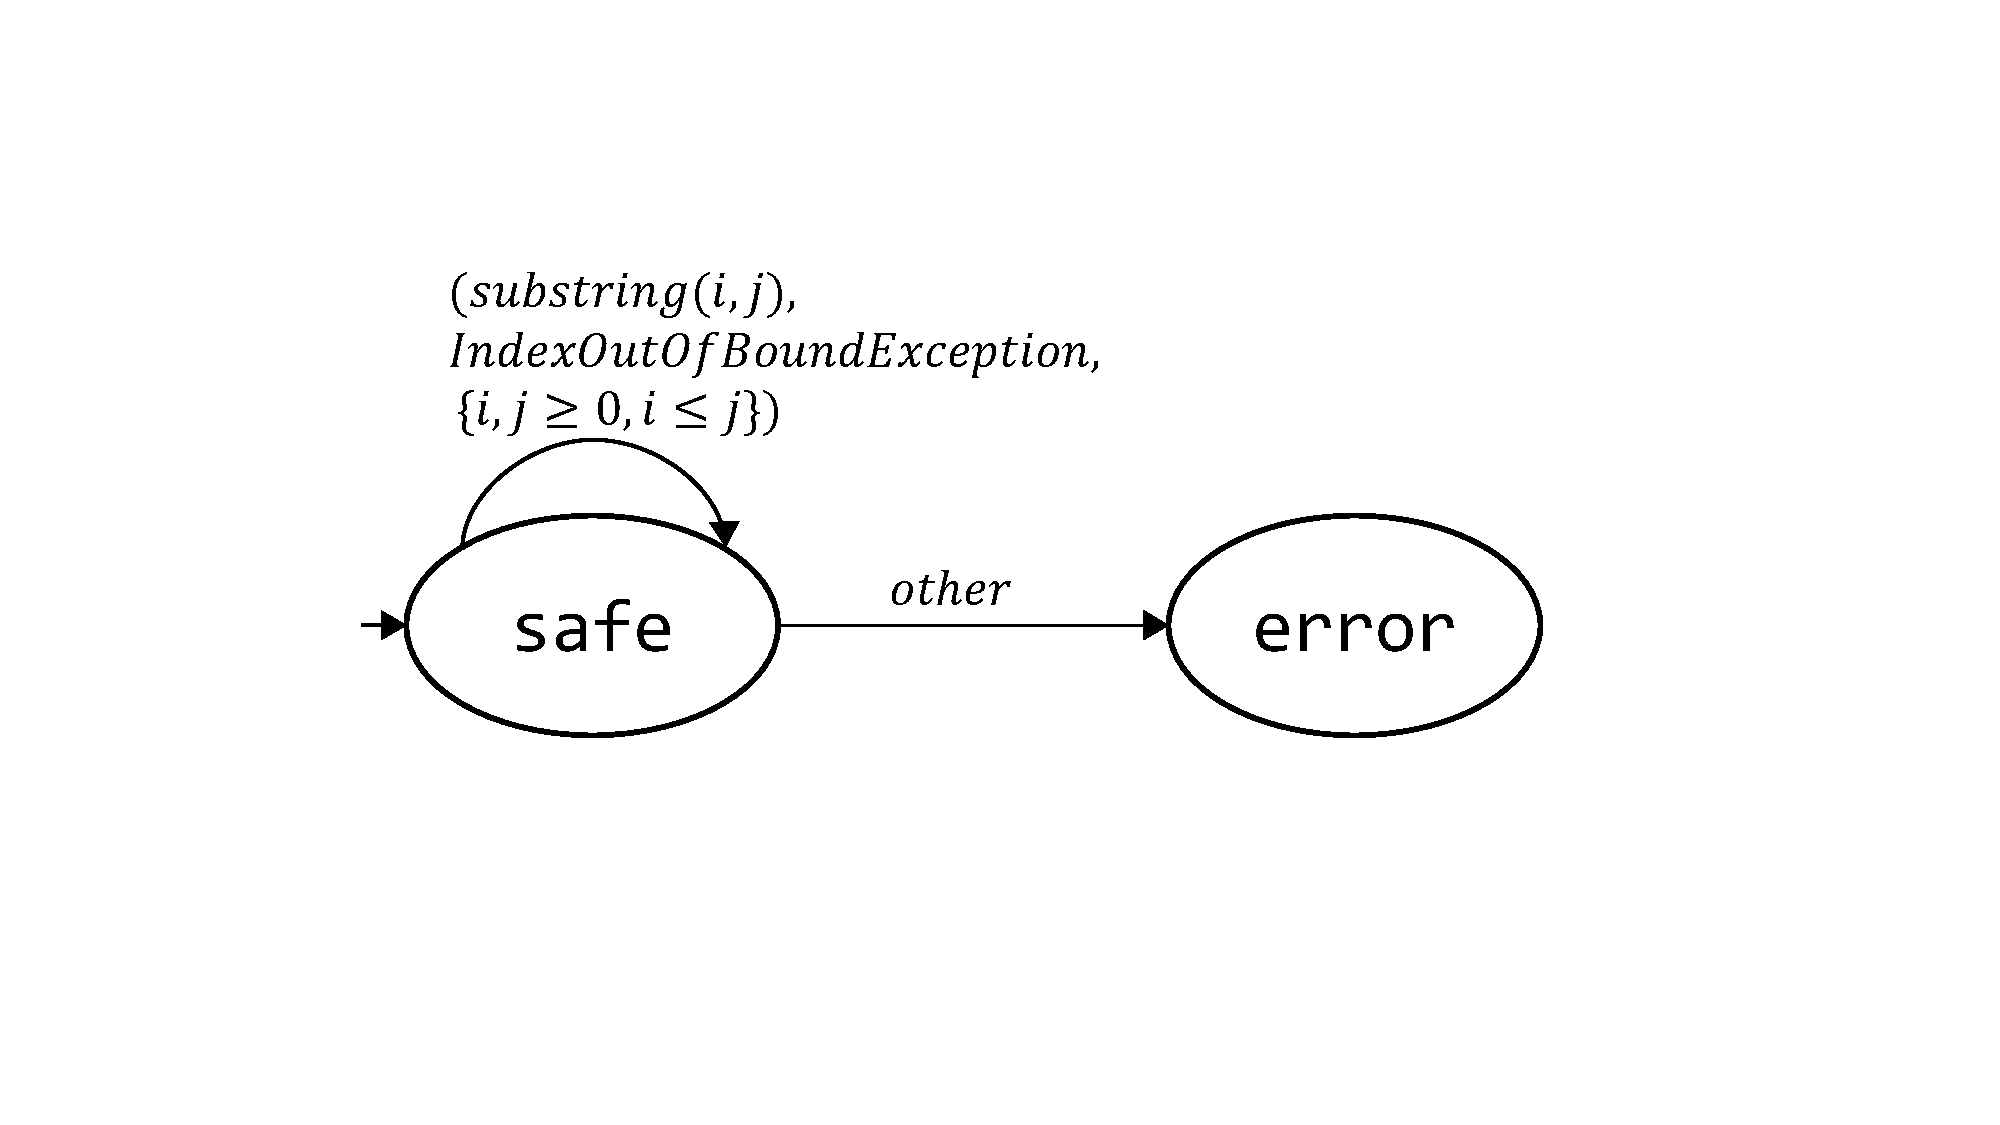
\includegraphics[scale=.25]{images/automataString.pdf}
\caption{Partial constraint representation model.}
\label{fig:constraintautomata}
\end{figure}


A partial constraint representation model is depicted in 
Figure~\ref{fig:constraintautomata}. It essentially specifies the constraints
that are associated with \code{substring} method and
\code{IndexOutofBoundException} exception that can be thrown by the method. A
complete model would have several such self-looping transitions corresponding to
other \java\ \code{String} API methods. The repairing mechanism gets triggered
when an exception is thrown while performing a string operation after at least
one of the constraints on the structure of the associated string is violated.
This is represented by the transition labeled by \code{other}. The patches
essentially support the same semantics identified by the transitions with the
help of \code{catch} blocks.

\section{Implementation}
\label{sec:implementation}

We implemented a prototype of \tool\ as described in \xref{sec:design} for
repairing runtime exceptions originating from unhandled \java\ \code{String}
APIs. Our end-to-end toolchain is completely automated and was written in
$\sim$$12.7K$ lines of \java. We leveraged the \soot~\cite{soot} framework for
bytecode analysis and instrumentation, and \infoflow~\cite{infoflow} for static
taint analysis.
We now briefly describe a few salient features of our implementation, which is
also available for download at \url{https://github.com/aritradhar/CLOTHO}.

\subsection{Taint Analysis}

\infoflow\ performs its taint propagation over \code{Units}, which are \soot's
intermediate representation of the \java\ source code. We extended the
\infoflow\ framework to a) enable seamless coupling with \soot, and b) determine
whether it is safe to patch a given \soot\ \code{Unit}. Specifically, we added
a mapping that retrieves \code{Unit}s for statements to be patched given a
specified method signature. This is relevant since the same statement, say
\code{int x = 1;} has the exact same representation even if it appears more
than once in a same method. We also added a utility method to determine if a
\code{Unit} must be patched if it lies along the path between a source and sink 
in the call graph (as generated by \soot).

\subsection{Interprocedural Exception Analysis}
\label{subsec:callChainLookUp}

\tool\ leverages \soot\ generated call graph to determine both inter- and
intra-method checked runtime exceptions (recall \xref{sec:tool:stage1}). \soot\
uses the \code{Trap} class to manage exception handling for both classes of
exceptions discussed above. Each \code{Trap} object has start, end and handler
unit.  We tagged every \code{Unit} in a \code{HashMap} if it belonged to an
existing \code{Trap}, so as to exclude it from instrumentation during the
repairing phase. \ignore{In the implementation we have added a switch to
\tool  where the users can turn of this analysis feature to look for already
handled exception. In such cases we call the patching as forced
patching.} \tool\ also provides an option of \textit{forced} patching by disabling
exception analysis and patching code irrespective of whether the exception
was handled or not. \note{Please check this. Made a few changes here.}

\subsection{Constraint Analysis}
\label{subsec:constraint analysis}

\tool\ makes a forward pass over the \code{Units} identified by the taint
analysis and other program analysis in the first phase to gather constrains over
string literals of interest (recall \xref{sec:tool:stage2}), and builds a
\code{HashMap} of \code{ConstraintDataType}, a custom data type to store and
evaluate these constrains. Specifically, each \code{ConstraintDataType} entry
stores four key parameters---the permissible prefixes, substrings, minimum and
maximum length---that specify constraints corresponding to a \code{String}
literal.

Constraint evaluation over these \code{ConstraintDataType} entries is done as
discussed earlier in Algorithm~\ref{algo:constraint}. However, if the gathered
constraints can not be satisfied statically, \eg\
\code{if(str.contains(userInput()))}, \tool\ instruments the bytecode before the
conditional statement with a static invocation to i) populate the corresponding
\code{ConstraintDataType} entry, and ii) recompute the permissible values of the
string object with already existing constraints (see Code
snippet~\ref{snippet:exCode2}).


\subsection{Optimizations}
\label{subsec:optimizations}

\tool\ performs a few other optimizations to improve the precision and quality
of the patches.

\subsubsection{Minimize constraint analysis}
\label{subsubsec:minimizeConstrintInstrumentation}

\tool\ collects constraints only for those string literals that may be involved
in a runtime exception. For example, if a string object does not involve API
methods that can throw runtime exception, then it is not required to collect and
evaluate constraints on them. This significantly reduces the number of
statements analyzed for instrumentation.
 
\begin{table*}[t]
% \setlength{\tabcolsep}{3pt}
\centering
\caption{\tool's accuracy results when applied to $30$ bugs in popular
open-source libraries.}
\caption*{
\scriptsize
\centering
\setlength{\tabcolsep}{3pt}
\begin{tabular}{ll|ll|ll}

$\mathcal{N}_{CG}$ & \# nodes in call graph & $\mathcal{T}$ & \# total cases in
test suite & $FCI$ & Flow Consistency Index\\

$\mathcal{N}_{Unit}$& \# \code{Units} analyzed & $\mathcal{F}_{P}$ & \# failed
tests in patched version w/o forced patching & $\mathcal{IC}_{NO}$
& Instrumentation w/o optimization (recall \xref{subsec:optimizations})\\

$\mathcal{S}_{U}$ & \# successful tests in unpatched & $\mathcal{F}_{P}^{*}$ &
\# failed tests in patched version w/ forced patching & $\mathcal{IC}_{WO}$ &
Instrumentation w/ optimization (recall \xref{subsec:optimizations})\\

$\mathcal{F}_{U}$ & \# failed tests in unpatched & $PPI$ & Patch Precision
Index & $\mathcal{RS}_{CE}$ & Cascaded exception exists
\end{tabular}
}

\scriptsize
\begin{tabular}{|l|c|l|r|r||r|c|r|c|c||r|c|r|r|c|}

\hline
\multicolumn{1}{|c|}{\textbf{API}} &
\multicolumn{1}{c|}{\textbf{BugID}} &
\multicolumn{1}{c|}{\textbf{Priority}} &
\multicolumn{1}{c|}{\textbf{$\mathcal{N}_{CG}$}} &
\multicolumn{1}{c||}{\textbf{$\mathcal{N}_{Unit}$}} &
%\multicolumn{1}{c|}{\textbf{$PPI$}} &
\multicolumn{1}{c|}{\textbf{$\mathcal{S}_{U}$}} &
\multicolumn{1}{c|}{\textbf{$\mathcal{F}_{U}$}} &
\multicolumn{1}{c|}{\textbf{$\mathcal{T}$}} &
\multicolumn{1}{c|}{\textbf{$\mathcal{F}_{P}$}} &
\multicolumn{1}{c||}{\textbf{$\mathcal{F}_{P}^{*}$}} &
\multicolumn{1}{c|}{\textbf{$PPI$}} &
\multicolumn{1}{c|}{\textbf{$FCI$}} &
\multicolumn{1}{c|}{\textbf{$\mathcal{IC}_{NO}$}} & %instrumentation with
%optimization
\multicolumn{1}{c|}{\textbf{$\mathcal{IC}_{WO}$}} & %instrumentation without
% optimization
\multicolumn{1}{c|}{\textbf{$\mathcal{RS}_{CE}$}}  % cascaded exception
%new added col
\\

\hline
\code{Aries} & \cite{ARIES1204} & Major &$3.5K$  & $129$ &
$18$ & $2$ & $20$ &  &  & $0.83$ &  & $42$ & $5$ &  \\

\code{Commons CLI1.x} & \cite{CLI193} & Critical & $3.2K$ & $53$ &
$14$ & $2$ & $16$ &  &  & $0.74$ & & $19$& $19$ &  \\

\code{Commons CLI2.x} & \cite{CLI46} & Major & $3.2K$ & $21$ &
$13$ & $3$ & $16$ & $3$ & $1$ & $0.62$ &$1$ & $13$ &$2$ & $\checkmark$\\

\code{Commons Compress} & \cite{COMPRESS26} & Blocker & $4.0K$ & $134$ &
$32$ & $1$ & $33$ &  &  & $0.74$ & & $46$& $4$ & \\

\code{Commons IO} & \cite{IO179} & Major & $3.3K$ & $125$ &
$27$ & $1$ & $28$ &  &  & $0.77$ & & $76$ & $1$ & \\

\code{Commons Lang} & \cite{LANG457} & Major & $5.1K$ & $240$ &
$16$ & $2$ & $18$ &  &  & $0.59$ & & $168$& $8$ &  \\

\code{Commons Math} & \cite{MATH198} & Major & $3.4K$ & $300$ &
$19$ & $2$ & $21$ & $2$ &  & $0.89$ &$1$ & $36$ &$2$ &  \\

\code{Commons Net} & \cite{NET442} & Major & $3.3K$ & $14$ &
$22$ & $1$ & $23$ &  &  & $0.84$ & & $6$ & $1$ & \\

\code{Commons VFS} & \cite{VFS338} & Major &$4.5K$ & $37$ &
$18$ & $1$ & $19$ &  &  & $0.65$ & & $20$ & $2$ &  \\

\code{Derby} & \cite{DERBY4748} & Major & $4.4K$ & $40$ &
$30$ & $2$ & $32$ &  &  & $0.46$ & & $47$ & $6$ &  \\

\code{Eclipse AJ Weaver} & \cite{EclipseBug432874} & Major & $20.6K$ & $50$ &
$17$ & $2$ & $19$ & $2$ & $2$ & $0.98$ & & $4$ & $1$ & $\checkmark$ \\

\code{Eclipse AJ} & \cite{EclipseBug333066} & Major & $25.0K$ &$39$ &
$14$ & $2$ & $16$ &  &  & $0.87$ & & $6$ & $1$ & \\

\code{FlexDK 3.4} &\cite{SDK14417} & Minor & $6.3K$ & $600$ &
$13$ & $2$ & $15$ &  &  & $0.74$ & & $207$ & $25$&  \\

\code{Hama 0.2.0} &\cite{HAMA212}  & Critical & $3.7K$ & $35$ &
$13$ & $1$ & $14$ &  &  & $0.55$ & & $28$ & $5$ &  \\

\code{HBase 0.92.0} &\cite{HBASE4481}  & Critical & $4.8K$ & $61$ &
$24$ & $1$ & $25$ &  &  & $0.83$ & & $13$ & $2$ &  \\

\code{Hive} &\cite{HIVE6986} & Trivial &$4.4K$ & $23$ &
$18$ & $1$ & $19$ &  &  & $0.75$ & & $8$ & $1$ &  \\

\code{HttpClient} &\cite{HTTPCLIENT150} & Major & $3.3K$ & $14$ &
$20$ & $3$ & $23$ &  &  & $0.89$ & & $6$& $1$ &  \\

\code{jUDDI} & \cite{JUDDI292} & Major &$3.2K$ & $70$ &
$28$ & $1$ & $29$ &  &  & $0.85$ & & $10$ & $2$ &  \\

\code{Log4j} & \cite{ApacheLog4jBug} & Major & $3.2K$ & $17$ &
$8$ & $3$ & $11$ &  &  & $0.74$ &  & $6$ &$1$ &  \\

\code{MyFaces Core} & \cite{MYFACES416} & Major  & $4.5K$ & $50$ &
$11$ & $3$ & $14$  &  &  & $0.83$ &  & $4$& $2$ &  \\

\code{Nutch} & \cite{NUTCH1547} & Major & $4.5K$ & $90$ &
$8$ & $3$ & $11$ &  &  & $0.68$ & & $8$ & $1$ &  \\

\code{Ofbiz} & \cite{OFBIZ4237} & Minor & $4.4K$ & $28$ &
$20$ & $3$ & $23$ & $3$ &  & $0.45$ &$1$ & $6$ &$1$ &  \\

\code{PDFBox} & \cite{PDFBOX467} & Major &$4.4K$ & $23$ &
$15$ & $3$ & $18$ &  &  & $0.87$ & & $8$ & $1$ &  \\

\code{Sling Eclipse IDE} & \cite{SLING3095} & Major & $4.5K$ & $58$ &
$5$ & $1$ & $6$ &  &  & $0.59$ &  &$39$ & $6$ &  \\

\code{SOAP} & \cite{SOAP130} & Major &$5.0K$ & $165$ &
$18$ & $3$ & $21$ & $3$ &  & $0.84$ & $1$ & $32$ & $5$ &  \\

\code{SOLR 1.2} & \cite{SOLR331} & Major & $11.0K$ & $200$ &
$12$ & $2$ & $14$ &  &  & $0.89$ &  & $25$ & $4$ &  \\

\code{Struts2} & \cite{WW650} & Major & $16.0K$ & $80$ &
$11$ & $2$ & $13$ &  &  & $0.76$ & & $25$ & $2$ &  \\

\code{Tapestry 5} & \cite{TAP51770} & Major & $6.2K$  & $71$ &
$17$ & $3$ & $20$ &  &  & $0.70$ & & $31$ &$5$ &  \\

\code{Wicket} & \cite{WICKET4387} & Major & $70.0K$ & $68$ &
$20$ & $3$ & $23$ &  &  & $0.81$ & & $16$ & $1$ & \\

\code{XalanJ2} & \cite{XALANJ836} & Major & $3.3K$ & $33$ &
$11$ & $3$ & $14$ &  &  & $0.72$ & &$13$ & $2$ & \\

\hline

\end{tabular}

\label{tab:results}
\end{table*}

\subsubsection{Minimize patch instrumentation}
\label{subsubsec:minimizePatchInstrumentation}

\tool\ makes a forward pass over all bytecodes to determine if a specific string
object is modified after it has been patched. If the object is not modified then
no further patching of statements capable of throwing \code{NullPointerException} exceptions is
required, since the constraint would have been satisfied in the beginning and it would be valid
as long as the variable is not changed. Similarly, when the API usage is same and none of 
the method parameters are changed, no further patching would be required. This reduces the 
total number of possible
instrumentation required. 

\section{Evaluation}
\label{sec:results}

We now present an evaluation of \tool. In \xref{sub:accuracy}, we evaluate
\tool's effectiveness by measuring the quality of patches and related
instrumentation required. We use the test suites bundled with the library itself
to determine if \tool\ generated patches violate any test case. We also measure
how the several optimizations (as described in \xref{subsec:optimizations})
affect the patches generated by \tool. In \xref{sub:overhead}, we measure the
relative performance and resource penalties incurred with \tool. In
\xref{sub:casestudies}, we describe our experiences with some of the major bugs
from our data set.

\ignore{
\myparagraph{Data Set} We mined bug repositories of several open-source
\java-based applications and selected $30$ bugs, majority of them being rated
either major, critical or blocking. \note{All of these bugs were very
recent and reported in the libraries which are widely used across products.
Moreover these bugs were specifically occurred in \code{String} APIs which fits
our problem definition.} These bugs involved usage of $64+$ different APIs from
\java's \code{String}, \code{StringBuffer}, \code{StringBuilder}, and Apache
\code{StringUtils} and Google Guava \code{StringUtils} classes.}

\myparagraph{Data Set} We mined bug repositories of several open-source
\java-based applications and libraries, and selected $30$ most recent
\code{String}-related bugs affecting the libraries, which are widely used across
several products. All bugs except one were rated either major, critical or
blocker. These bugs involved usage of over $64$ APIs from \java's
\code{String}, \code{StringBuffer}, \code{StringBuilder}, Apache
\code{StringUtils} and Google Guava \code{StringUtils} classes.

\myparagraph{Experimental Setup} All our experiments were performed on a laptop
with $2.9$ GHz dual core Intel i$5$ CPU, $8$ GB RAM and running Microsoft
Windows $8.1$. The JDK (v$1.7$) itself was provisioned with $2$ GB heap space.
\ignore{We used JDK v$1.7$ running with $2$ GB of allocated heap space.}
% All bug reproduction was done on Eclipse Juno IDE.
We used \infoflow\ (snapshot from May 2014)
for static taint analysis, and \soot\ v$2.5.0$ for bytecode analysis and
instrumentation.

\subsection{Accuracy}
\label{sub:accuracy}

We evaluate the precision of the patch and the effectiveness of \tool\ as
described below.

\begin{mylist}

\item \textbf{Effectiveness of the patch}: A software patch is \emph{effective}
if it does not violate any existing test case from the software's test suite.
Thus, we determined the effectiveness of \tool\ generated patches by running
them against the benchmark's existing test suites. Table~\ref{tab:results} lists
$30$ real-world bugs mined from bug repositories of popular open-source
libraries. Column $\mathcal{T}$ lists the total number of cases in the test
suite, while $\mathcal{S}_{U}$ and $\mathcal{F}_{U}$ lists the number of
successful and failed cases in unpatched version, respectively. Columns
$\mathcal{F}_{p}$ and $\mathcal{F}_{p}^{*}$ represent the count of failed test
cases without and with \tool{}'s forced patching,
% (to address cascaded exceptions)
respectively.

We wrote a driver program to recreate the bug, and then applied \tool\ on the
library to patch it. We observed that \tool\ without any optimizations patched
$25$ of the $30$ offending bugs in our benchmarks, an effectiveness of over
$83\%$. With forced patching enabled,
% (to overcome cascaded exceptions arising from \code{String} operations)
\tool\ successfully patches all but two benchmarks, thereby raising its
effectiveness to over $93\%$. Note that even the force patched versions of
\code{Commons CLI2.x} and \code{Eclipse AJ Weaver} fail test cases. We observed
that in both benchmarks the offending test case throws a non-\code{String}
related \textit{cascaded} exception that \tool\ could not patch, thereby
resulting in failed test scenarios.

\item \textbf{Precision of the patch}: Precision of a patch is governed by the
similarity between a \tool\ generated patch and the developer's fix for the same
bug. We define \textbf{Patch Precision Index (PPI)} as a measure of the
precision of the patch. $$PPI =
\frac{\#~Constraints_{\tool}}{\#~Constraints_{Developer}}$$
% * \frac{\#~LOC_{Developer}}{\#~LOC_{\tool}} *
% \frac{Output_{\tool}}{Output_{Developer}}$$
% 
Specifically, PPI compares the similarities in constraints in \tool's patch
against the developer's version, thereby considering the core logic to construct
an effective patch. \tool\ analyzes and registers the constraints that are
related to only \code{String} objects, thereby ensuring that PPI is also
influenced by constraints on \code{String} objects alone. If \tool's patch has
fewer constraints than the developer's fix, the PPI will be less than $1$. In
contrast, PPI greater than $1$ indicates that \tool\ generates many more
constraints than those in the developer's fix. Thus, a PPI closer to $1$ is
desirable. PPI can be computed automatically, since \tool\ already generates a
list of constraints (in the form of bytecodes), and static analysis of the
developer's patch can provide the same.
%\note{Some grammatical issue. Please fix.}

Table~\ref{tab:results} lists the PPI for the benchmarks in our set. We note
that PPI is \textgreater\ $0.7$ for over $73\%$ of the benchmarks. This high PPI
across several benchmarks indicates the number of \code{String} constraints
considered by \tool\ is close to that of the developer's fix. This is a direct
evidence that \tool\ generates patch closer to program specification and hence
comparable to an actual patch.\ignore{two things:
(i) the conditional statements involved in the developer's bug fix includes a
high number of \code{String} operations, and (ii) \tool\ correctly matches and
fixes errors in several of these \code{String} operations} PPI for the remainder
of the benchmarks was observed to be lower, \ie\ \textless\ $0.7$.\ignore{ On
manual inspection of the concerned bugs, we noted that the constraints in the
specific conditional statement involved several other data types other than
\code{String}. Since \tool\ operates only over \code{String} objects, the
effective PPI reduces.} On manual inspection of the offending bytecodes, we
observed that \tool\ generated constraints on \code{String} conditionals were
very similar to the developer's fix, thereby confirming \tool's high precision
in generating patches.

\note{\todo{What is the PPI if we only compare \code{String} constraints?}}

Note that the taint analysis works only when sources and sinks are defined.
Since our library benchmarks have no notion of sources or sinks, \tool's
bytecode analysis of the libraries does not involve the taint analysis phase.
However, even without taint analysis, \tool's patches are of high quality, as
indicated by the high PPI.

\begin{table}[t]
\centering
\caption{Precision results for taint analysis.}
\scriptsize
\begin{tabular}{|l|r|r|r|}
\hline
\multicolumn{1}{|c|}{\textbf{Application}} &
\multicolumn{1}{c|}{\textbf{KLOC}} &
\multicolumn{1}{c|}{\textbf{Total paths}} &
\multicolumn{1}{c|}{\textbf{Tainted paths}}\\

\hline
\code{Checkstyle}& $58.0$ & $1977$ & $88$\\
\code{Jazzy Core}& $4.9$ & $270$ & $26$\\
\code{JEdit}& $4.3$ & $185$ & $22$\\

\hline
\end{tabular}

\label{tab:taintAnalysis}
\end{table}

\item \textbf{Precision of taint analysis}: \tool\ leverages off-the-shelf tools
(\infoflow) to perform the taint analysis. We measure precision of our choice of
tool by measuring the number of statements in the analyzed code that are deemed
unsafe to patch. Since we could not measure the precision of taint analysis on
the library benchmarks (for reasons discussed earlier), we select $3$ diverse
applications and apply \tool\ in its entirety to obtain a measure of the
precision of the taint analysis. Specifically, for each application we provided
a set of sources, sinks and taint propagators to \infoflow, which listed the
total number of tainted paths, \ie\ paths from a sensitive source to a sink and
thus must not be patched. Table~\ref{tab:taintAnalysis} lists the results. We
observe that the total number of tainted paths is less than $12\%$ across the
applications.

\myparagraph{Threats to validity} Note that \tool\ is dependent on \infoflow\
for achieving precision about the points of instrumentation. However,
\infoflow\ currently has a major limitation---it does not support taint
analysis for multi-threaded programs. Moreover, since it is still under active
development, we observed that when applied to certain applications, \infoflow\
consumed inordinate amounts of memory and crashed. Thus, \tool's precision is
limited by the accuracy of its dependencies. 

\item \textbf{Already handled exceptions}: \tool\ analyzes the call graph to
determine if a potential runtime exception throwing statement is handled higher
up in the call chain or in the same method. In such cases \tool\ must abort the
patching effort considering that the exception is caught with exact exception
type or its base type. This is required else patching will disrupt the normal
control flow of the program.

We measure the extent of this optimization, which prevents disruption of the
control flow, using the \textbf{Flow Consistency Index (FCI)} that is calculated
as $FCI = n$, where $n$ is the number of exceptions in the application that
must be ignored \tool\ for forced patching of the bug. Note that $FCI \ge 0$,
and a lower value of $FCI$ is desirable. We observe that patching four bugs
required \tool\ to ignore at most one exception; rest required no changes.

\item \textbf{Cascaded exceptions}: A cascaded exception arises if the
\tool-generated patch creates objects that when used as inputs to other \java\
APIs result in further exceptions. \tool\ is prone to cascading exceptions
because of the limitation of its intra-procedural analysis and a simple
constraint evaluation mechanism. However, \tool's constraint solver is pluggable
and a more sophisticated third party solvers can easily be integrated.
Specifically, cascaded exceptions may arise if the patch generates \code{String}
objects that represent a malformed string. Further, if we keep the optimization
in \xref{subsubsec:minimizePatchInstrumentation}, then cascaded failures may
occur even for subsequent \code{String} APIs handling the malformed
string following the point of patching. If the optimization is turned
off, \tool\ will automatically patch all relevant \code{String} APIs and thus
handle all cascaded failures involving malformed \code{String} objects.
We observe that two benchmarks throw cascaded exceptions even after being
repaired. The cascading was one level deep and triggered exception in another
non-\code{String} code (and thus unpatched), which caused the application to
crash.

\end{mylist}

%already given at implementation section
\ignore{Detailed evaluation for each of the bugs in our data set is available at
\url{https://github.com/aritradhar/CLOTHO}.}

\begin{figure*}[t]
\centering
\begin{tabular}{ccc}
\subfloat[Variation in call graph analysis time with size of call
graph.\label{fig:perf:callgraph}]
{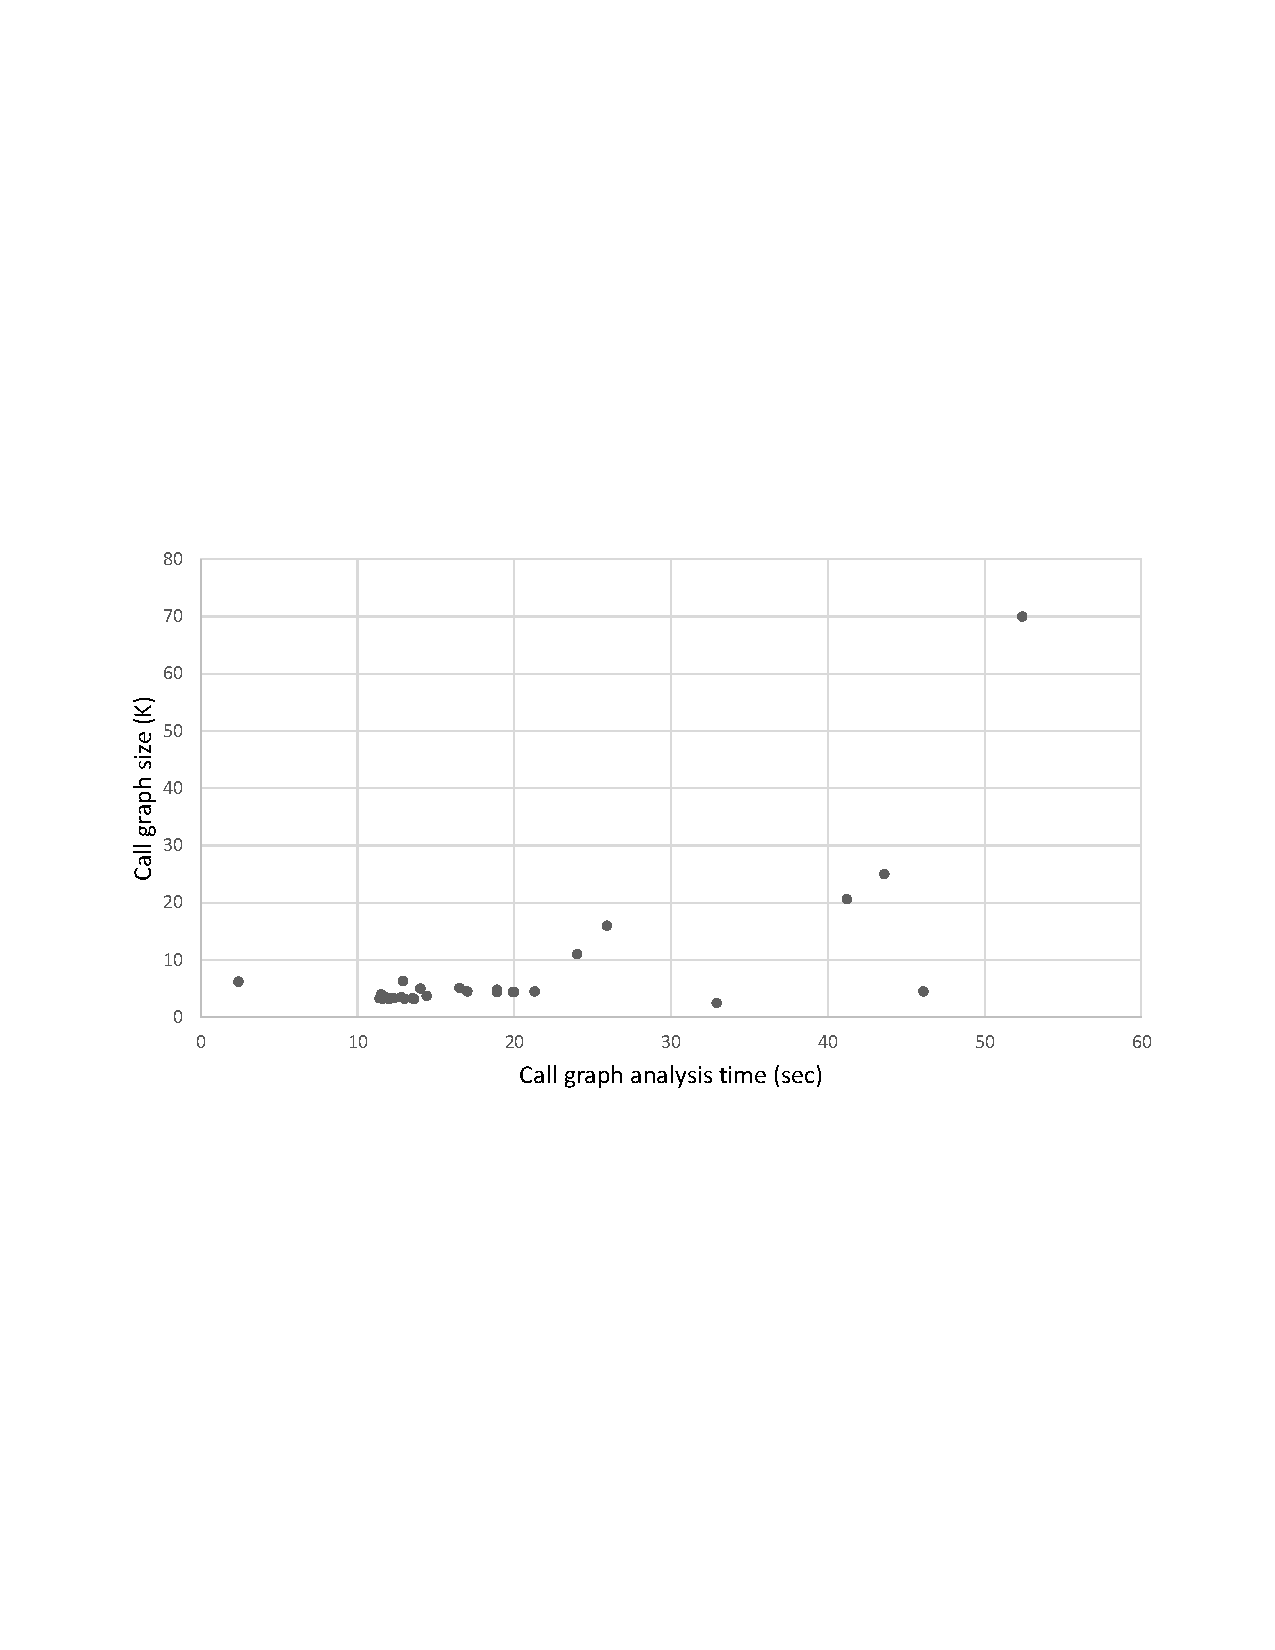
\includegraphics[width=.3\linewidth]{images/CgSizeVsTime.pdf}}
\hfill
&
\subfloat[Variation in static constraint analysis time with number of
constraints.\label{fig:perf:constraints}]
{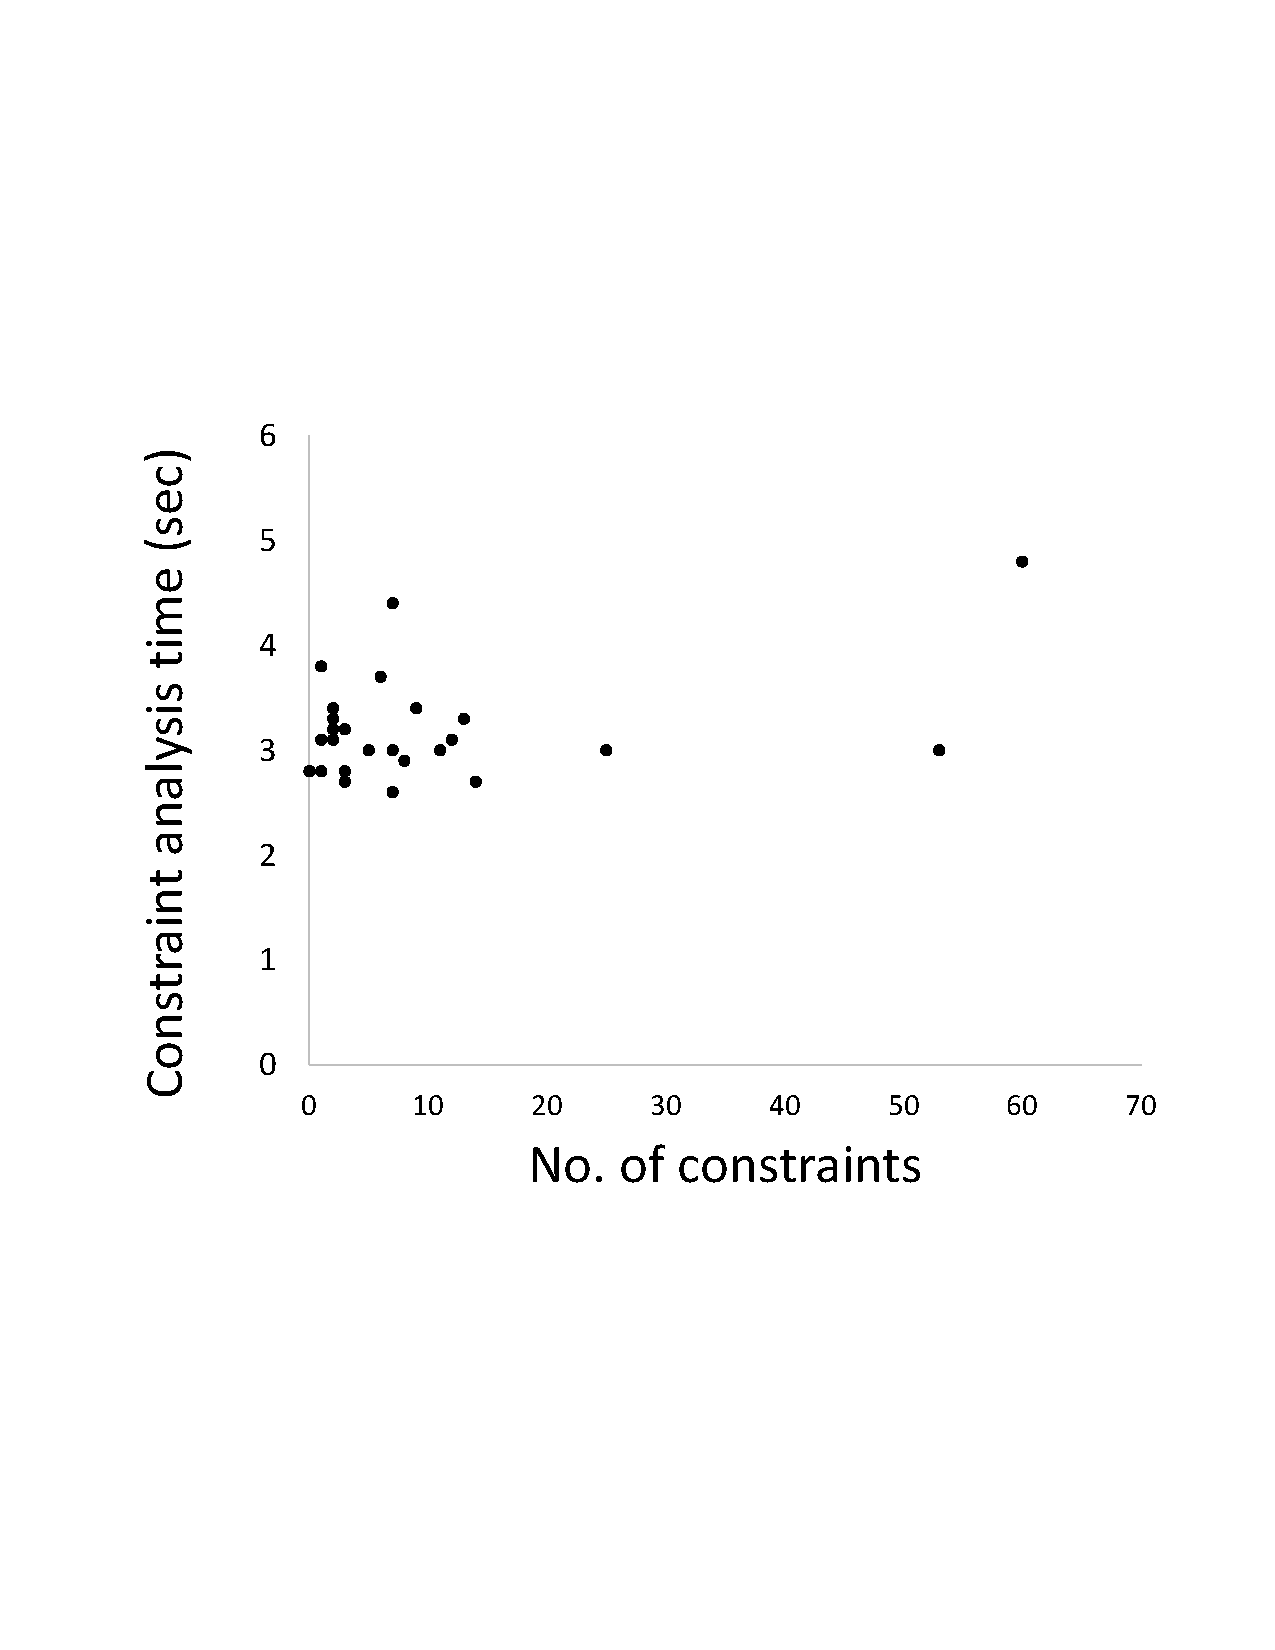
\includegraphics[width=.3\linewidth]{images/ConstraintsVsTime.pdf}
}
\hfill
&
\subfloat[Variation in instrumentation time with \code{Units} to be
instrumented.\label{fig:perf:units}]
{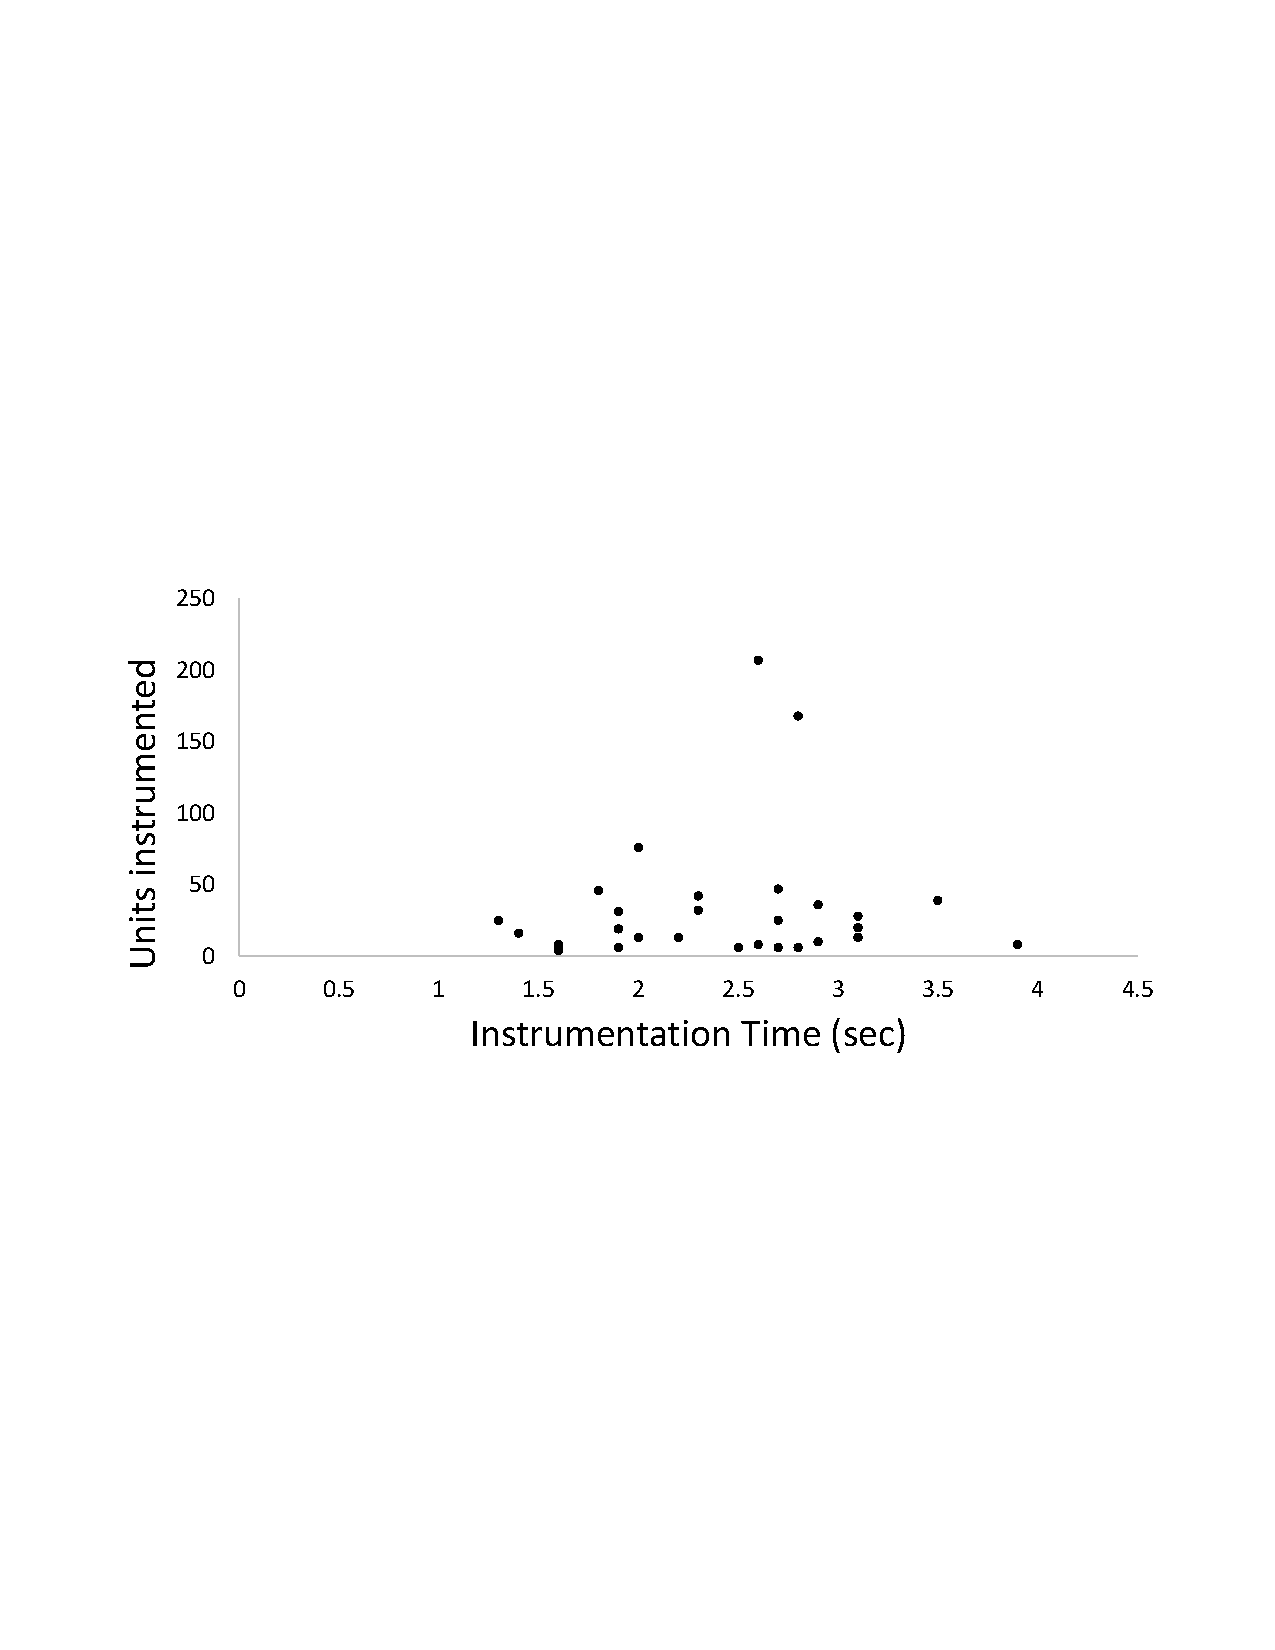
\includegraphics[width=.3\linewidth]{images/InstrumentationVsTime.pdf}}
\hfill
\\
\end{tabular}
\caption{\tool\ evaluation.}
\end{figure*}

\subsection{Overhead}
\label{sub:overhead}

We measure the overhead of \tool\ across different metrics identified below.

\begin{mylist}

 \item \textbf{Execution overhead}: We randomly selected and patched $5$
libraries (Apache Tapestry, Apache Wicket, Eclipse AspectJ Weaver, Hive and
Nutch) from Table~\ref{tab:results} to determine the execution overhead of the
patched class files. We observed that \tool\ reports an average overhead of
$\sim$$2.32\mu$s per call across the $5$ benchmarks for $50K$ runs of the
patched functionality in both the developer's version and \tool's patched
library. The maximum absolute overhead was observed for Hive at $\sim$$3.96\mu$s
per call. The above overhead is imperceptible at human response time scales.

 \item \textbf{Call graph}: The size of the call graph directly governs the time
and memory consumption for \tool. Figure~\ref{fig:perf:callgraph} shows the
results for the benchmarks analyzed from our data set. The overall analysis
time was under a minute for all the benchmarks. We observed that even for a call
graph of $\sim$$70K$ nodes (for \code{Wicket}), \tool\ required just $52.4$s
and $210$MB memory.

 \item \textbf{Constraint set}: \tool\ performs an exhaustive multi-pass
analysis to gather and evaluate the set of constraints for generating patches. A
higher number of constraints and their complexity increases the duration of
\tool's analysis. Figure~\ref{fig:perf:constraints} compares the time required
for static constraint collection and evaluation with an increasing number of
constraints for the benchmarks used in our data set. We observe that across
all the benchmarks used, \tool\ required at most $\sim$$5$s for collecting and
evaluating the constraints.

\item \textbf{Instrumentation overhead}: \tool\ performs bytecode
instrumentation for actual patching. Figure~\ref{fig:perf:units} shows the
variation in instrumentation time with increasing number of \code{Units} to be
patched. We observe that even without optimization discussed in
\xref{subsec:optimizations}, \tool\ takes under $4$s to instrument all
\code{Units} across all benchmarks. We believe that this time would be even
less with the optimizations enabled, which significantly decrease the number of
\code{Units} to be instrumented, and is evident in Table~\ref{tab:results} where
column $\mathcal{IC}_{WO}$ is much less than $\mathcal{IC}_{NO}$.

\end{mylist}

\subsection{Case studies}
\label{sub:casestudies}

We now report on experiences gained when using \tool\ to patch several of the
bugs reported in Table~\ref{tab:results}.

\begin{mylist}

 \item The bug~\cite{ARIES1204} as reported in the repository for Apache Aries
cited String related issues. However, our investigation showed that the bug was
actually in the ASM framework that was invoked by Aries, and not in the Aries
framework as originally reported. Thus, we patched the particular ASM methods
containing the bugs, and retested it with the Aries framework to ensure
conformance.

 \item The bug in Commons Math~\cite{MATH198} had a bug related to incorrect
formatting of the input string. However, it threw a completely irrelevant
exception (\code{IndexOutOfBound}) instead of the \code{NumberFormatException},
which contains the information of the malformed string. The \tool-generated
patch fixes the undesirable behavior.

 \item The bug in OfBiz~\cite{OFBIZ4237} throws a custom shutdown exception,
when in fact it should throw a \code{StringIndexOutOfBoundsException} due to a
\code{substring} invocation with incorrect bounds. This ultimately causes the
library to throw some high priority exception and ultimately crash if not handed
properly by the application. The patched version of the library catches the
correct exception.

 \item The code to trigger bugs in some libraries, including Apache Commons
Compress, Commons Lang, Commons Math and Ofbiz, each had string operations
wrapped in \code{try-catch} block that were handled by \code{Exception} class,
\ie\ the base type of all exceptions. However, \tool\ checks for already
handled runtime exceptions during its call graph analysis, and thus did not
patch the bugs. We turned off the call graph analysis module to force \tool\ to
generate the relevant patch for the bug.

 \item We also noticed several instances where the developer code does not
follow proper programming practices regarding exception handling. For example,
the SOAP bug~\cite{SOAP130} was reported for a faulty \code{substring} call that
threw a \code{StringIndexOutOfBoundsException}. The entire method was wrapped in
a \code{try-catch} that included the faulty substring call along with other
servlet operations. However, the \code{catch} block handled the generic
\code{Exception}, which is the base class for all exceptions. Thus, both the
servlet exceptions and the \code{IndexOutOfBoundException} from the
\code{substring} call were handled in a generic fashion. \tool's patched library
ensures that exceptions originating from the \code{substring} call are handled
properly.

\end{mylist}
\section{Discussion}
%\section{Limitations and Remedies}
\label{sec:discussion}

%\subsection{Weaknesses and Remedies}
%\label{sec:discussion:limitation}
In this section we discuss the weaknesses of \tool\ and also propose
remedies to overcome them.

\paragraph{Focus on String APIs} \tool\ is heavily directed towards repairing 
handling \code{String} objects and API
exceptions. While this may seem to be a limitation, we believe that \tool's
strength lies in the fact that it mines contextual data about runtime exceptions
related to \code{String} objects that helps development of intelligent patches.
Moreover, \tool's technique is generic and can be ported to any other class of
\java\ APIs. We leave this extension for the future.

\paragraph{Lack of guarantee regarding patch correctness} \tool attempts to generate 
precise patches considering the program context which avoids
cascading exceptions to a great extent producing the intended behavior in case
of failures. However, it still cannot give guarantees about elimination of cascading
exceptions, particularly when there are heavy object dependencies in the program.
In the future, we plan to support \tool\ with program invariants that would ensure 
acceptable behavior. The invariants can be specified by a programmer or can be
automatically generated with the help of training runs.

\paragraph{Handling of limited constraints} The constraint data store used by \tool\
is easy to build as it captures
limited number of fairly simple \code{String} characteristics which are used to
generate patching \code{String} objects. This approach may not be adequate particularly
if the program contains a large number of complex constraints. The quality of
\tool's patches would generally depend on the nature of its constraint solver,
which is pluggable. \tool's current solver is simple and can efficiently
handle a limited number of simple constraints. A more sophisticated off-the-shelf solver may improve
the repair quality. However, the current evaluation of the tool
on several library APIs described in Section~\ref{sec:results} indicates that the constraints that exist
in practice are normally less complex and are limited in number. \note{Please check this section.}


\ignore{
\paragraph{Focus on String APIs} \tool's major limitation arises from the fact that it
is heavily directed towards repairing handling \code{String} objects and API
exceptions. While this may seem to be a limitation, we believe that \tool's
strength lies in the fact that it mines contextual data about runtime exceptions
related to \code{String} objects that helps development of intelligent patches.
Moreover, \tool's technique is generic and can be ported to any other class of
\java\ APIs.

\tool generates precise patches considering the program context which avoids
cascading exceptions to a great extent producing the intended behavior in case
of failures. However, it still cannot give guarantees about elimination of cascading
exceptions, particularly when there are heavy object dependencies in the program.




\subsection{Remedy}
\label{sec:discussion:remedy}

\note{In the previous section we discuss about the major limitation of \tool\
i.e. it is rather focused on only \code{String} objects. But one key point here
is that the limitation exists because of the current implementation of \tool.
This technique can be applied to objects other than \code{String} but requires
rigorous study to understand the characteristics (behavior and types of
exceptions thrown) associated to the APIs related to that object. \tool
calculates patch by analyzing constrains. Proper study is required to understand
the constraints associated to the object to apply \tool.}

\note{The quality of \tool's patches also depends on the nature of the
constraint solver, which is pluggable. A more sophisticated solver may improve
the quality of program repair, and we leave comparison of different solvers for
future work. }

\subsection{Future Works}
\label{sec:discussion:futureWorks}

Our study shows that \tool\ can handle programs that are real, and can produce
patches efficiently. Motivated by the results of our study as well as by the
research conducted by other researchers, we intend to extend \tool\ in the
future by adding support for other \java\ APIs and also by adding more
intelligence to the process of patch generation.
}



\section{Related Work}
\label{sec:relatedWorks}

\subsection{Recent Works on Data Structure Repairing}
\label{subsec:RecWorksDataStructure}

Automated data-structure repairing techniques are there in the literature for a
while. In the papers~\cite{conf/oopsla/DemskyR03, Demsky03automaticdata,
conf/icse/DemskyR05, conf/issre/DemskyR03, conf/issta/DemskyEGMPR06} the authors
mostly concentrated on specific data-structures like \emph{FAT-32}, \emph{ext2},
\emph{CTAS} (a set of air-traffic control tools developed at the NASA Ames
research center) and repairing them. The authors represented a specification
language by which they able to see consistency property these data-structure.
Given the specification, they able to detect the inconsistency of these
data-structures and repair them.
The repairing strategy involves detecting the consistency constraints for the
particular data structure, for the violation, they replace the error condition
with correct proposition. In the paper~\cite{conf/icse/DemskyR05}, the authors
Brian Demsky and Martin C. Rinard proposed repair strategy by goal-directed
reasoning. This involves translating the data-structure to a abstract model by a
set of model definition rules. The actual repair involves model reconstruction
and statically mapped it to a data structure update. In their
paper~\cite{conf/oopsla/2007} authors Bassem Elkarablieh, Sarfraz Khurshid, Duy
Vu, Kathryn S. McKinley proposed the idea to statically analyze the data
structure to access the information like recurrent fields and local fields. They
used their technique to some well known data structures like singly linked list,
sorted list, doubly liked list, N-ary tree, AVL tree, binary search tree,
disjoint set, red-black tree, Fibonacci heap etc.

\subsection{Works on Software Patching}
\label{subsec:RecWorksSoftPatch}

In their paper~\cite{conf/sosp/PerkinsKLABCPSSSWZER09}, authors Jeff H.
Perkins, Sunghun Kim, Samuel Larsen, Saman P. Amarasinghe, Jonathan Bachrach and
Michael Carbin, Carlos Pacheco, Frank Sherwood, Stelios Sidiroglou, Greg
Sullivan, Weng-Fai Wong,Yoav Zibin, Michael D. Ernst and Martin C. Rinard
presented their \emph{Clear view} system which works on windows x86 binaries
without requiring any source code. They used invariants analysis for which they
used Daikon~\cite{journals/scp/ErnstPGMPTX07}. They mostly patched security
vulnerabilities by some candidate repair patches.

Fan Lon et al in their paper~\cite{conf/pldi/LongSR14} presented their new
system \emph{RCV} which recovers applications from divide-by-zero and
null-deference error. Their tool replaces \emph{SIGFPE} and \emph{SIGSEGV}
signal handler with its own handler. The approach simply works by assigning zero
at the time of divide-by-zero error, read zero and ignores write at the time of
null-deference error. Their implementation was on $x86$ and $x86-64$ binaries
and they also implemented a dynamic taint analysis to see the effect of
their
patching until the program stabilizes which they called as \emph{error
shepherding}.

\subsection{Genetic Programming, Evolutionary Computation}
\label{subsec:RecWorksGeneric}

Reserch works on program repair based on genetic programming and evolutionary
computation can be found in the paper of Stephanie Forrest, ThanhVu Nguyen,
Westley Weimer and Claire Le Goues~\cite{conf/gecco/2009g} and Westley Weimer,
Stephanie Forrest, Claire Le Goues, ThanhVu
Nguyen~\cite{journals/cacm/WeimerFGN10} respectively. In the papers, the authors
used genetic programming to generate and evaluate test cases. They used their
technique on the well known Microsoft Zune media player bug causing the
application to freeze up.



\section{Conclusion and Future Work}
\label{sec:conc}

Running programs may crash unexpectedly due to vulnerabilities in the code and
malformed data.
The cost associated with such crashes can be vary with the criticality of the
applications. Therefore, it is hardly a surprise that automatic program
repairing has been an actively researched area over the past decade.
In this work, we have presented a novel program repairing technique, and a tool
\tool\ based on it which employs hybrid program analysis to protect a running
program from failures originating from string-handling errors leading to a
program crash.
Our choice of \java\ \code{String} APIs is driven mainly by the popular usage of
string objects and bugs associated with them.
By focusing on a specific data type, and taking the program context into
account, \tool\ can develop patches that are precise and  semantically close to
the ones developed by the developers.
Hence, when the patches are activated, the program exhibits a behavior which is
close to the intended program behavior.

%this part is now in discussion section
Our study shows that \tool\ can handle programs that are real, and can produce
patches efficiently. Motivated by the results of our study as well as by the
research conducted by other researchers, we intend to extend \tool\ in the
future by adding support for other \java\ APIs and also by adding more
intelligence to the process of patch generation.


% \acks

% \clearpage

%\raggedright
\small
%\bibliographystyle{abbrvnat}
\bibliographystyle{plain}
\bibliography{paper}

\end{document}
